% % Adjust chapter counter for skipped chapters 2-4
% \setcounter{chapter}{4}
\chapter[Resilient Trust--Aware Distributed Observer Design for Connected Vehicle Platoons]{Resilient Trust--Aware Distributed Observer Design for Connected Vehicle Platoons}\label{chp5_chap}
% \chaptermark{Resilient Trust--Aware Distributed Observer Design for Connected Vehicle Platoons}

\objectif{This chapter proposes a trust-aware distributed observer for vehicle platoons that maintains resilient state estimation under cyberattacks. 
A behavioral divergence metric evaluates the reliability of shared data, forming a dynamic neighbor set used to adapt observer's weighting gains. 
Stability conditions are derived via Lyapunov analysis. 
Simulations under bogus, replay, and DoS attacks demonstrate robust performance and stable platoon behavior.
}

%%%%%%%%%%%%%%%%%%%%%%%%%%%%%%%%%%%%%%%%%%%%%%%%%%%%%%%%%%%%%%%%%%%%%%%%%%%%%%%%%%%%%%%%%%%%%%%%%
\section{Introduction}
%%%%%%%%%%%%%%%%%%%%%%%%%%%%%%%%%%%%%%%%%%%%%%%%%%%%%%%%%%%%%%%%%%%%%%%%%%%%%%%%%%%%%%%%%%%%%%%%%

\subsection{General introduction}
\vspace*{-0.3pt}
The rapid development of autonomous and connected vehicles has introduced new opportunities to improve road safety, traffic flow, and fuel efficiency. In vehicle platoons-where multiple vehicles coordinate through vehicle-to-vehicle (V2V) communication-accurate distributed state estimation is essential for maintaining stability and efficiency. Each vehicle must reconstruct both its own and others' states using locally sensed data and information exchanged with neighbors. However, this distributed structure also exposes the system to cyber and communication attacks that can disrupt coordination or compromise state estimation~\citep{Ali_book}. \\
%
Traditional estimation and control methods generally assume all vehicles are cooperative and trustworthy, which is unrealistic in adversarial environments~\citep{Shengya_HG}. Malicious or faulty agents can transmit falsified information, causing estimation errors that propagate through the network. Consequently, resilient estimation strategies capable of identifying and isolating untrustworthy data have become a key research direction in cyber-physical systems (CPS) and distributed multi-agent systems (DMAS).\\
%
Existing work on secure estimation and fault detection can be categorized into three main families:
\begin{itemize}
    \item {\it Observer-based detection:} compares model-predicted states with sensor measurements to identify anomalies \cite{Huy_LCSS,2_obs_Angelo}. These methods are effective for detecting deviations but may propagate errors if compromised neighbors provide false data.
    %--
    \item {\it Consensus-based detection:} relies on cross-validation among agents to identify inconsistent information \cite{Guitao_multi_mesure}. While robust under the assumption that most agents are trustworthy, their performance degrades under large-scale coordinated attacks.
    %--
    \item {\it Trust-based detection:} assigns reliability scores to neighboring agents based on behavioral or statistical consistency. Physical-signal approaches use device fingerprints for authentication \cite{trust_physic_connecte}, while statistical approaches compare communicated data against locally observed behaviors \cite{Wang_2021}. These methods improve resilience by filtering unreliable inputs before consensus or estimation steps, but they typically require significant computational resources or long-term historical data-making real-time adaptation challenging for dynamic platoons.
\end{itemize}
%
Mitigation strategies in the literature often depend on attack detection results. Some switch to fallback modes (e.g., CACC to ACC), while others incorporate trust scores directly into control to down-weight suspicious data \cite{self_belive,Enhancing_control_trust}. The latter provides finer control adaptation but relies heavily on accurate and timely trust evaluation. To overcome these limitations, we propose a trust-aware distributed observer framework for vehicle platoons. The framework continuously evaluates the trustworthiness of communicated data by comparing reported and predicted behaviors, dynamically adjusting observer weights according to each neighbor's trust score. This mechanism ensures reliable estimation even under cyberattacks or communication faults.

The main contributions of the paper can be summarized in the following items:
\begin{itemize}
    \item A formal definition of the resilient distributed state estimation problem for connected vehicles under adversarial conditions.
    \item A behavioral trust model that quantifies each agent's reliability and constructs a dynamic trusted neighbor set.
    \item A trust-informed distributed observer with provable stability guarantees, validated through simulations under multiple attack scenarios.
\end{itemize}

By integrating detection, mitigation, and estimation within a unified trust-based layer, the proposed method improves the resilience and stability of cooperative vehicle systems.

%The remainder of this paper is organized as follows. Section \ref{sec_vehiclemodel} describes the vehicle model. Section \ref{sec_Distributed Observer} introduces the distributed observer design. Section \ref{sec_trust_score} presents the trust framework and trust-weight-based adaptation. Section \ref{sec_Weigth_Design} presents the weight design and the stability analysis. Section \ref{sec_simulation} validates the proposed approach through simulation studies under multiple attack scenarios, followed by conclusions and future work in Section \ref{sec_conclusion}.

% Connected and autonomous vehicle platoons depend on coordinated state estimation to maintain safety, efficiency, and string stability. Each vehicle must estimate its own and neighboring states using a combination of onboard sensor data and vehicle-to-vehicle (V2V) information. However, this distributed structure introduces vulnerabilities: a single malicious or faulty agent can send incorrect information, leading to degraded estimation, unsafe distances, or even collisions. Ensuring resilient estimation against such disruptions is therefore crucial.

% Conventional distributed observers typically assume that all participating vehicles behave reliably. In practice, communication channels are exposed to cyberattacks, and data integrity cannot be guaranteed. Recent trust-based approaches evaluate the reliability of information sources, but they often rely on static weighting or historical patterns, which limits responsiveness in dynamic traffic conditions. Moreover, most existing frameworks treat trust as an external metric, rather than integrating it directly into the estimation process.

% To overcome these limitations, this paper introduces a trust-integrated distributed observer for vehicle platoons. The method uses a behavioral divergence metric that measures the inconsistency between each vehicle's reported states and its predicted physical behavior. Based on this metric, trust scores are continuously updated and used to construct a trust-adaptive neighbor set, which directly governs the observer's weighting matrix. This dynamic adaptation enables the platoon to automatically reduce the influence of untrustworthy agents while preserving cooperation among reliable vehicles.

% The main contributions are summarized as follows:

% Trust Model: A novel behavioral divergence-based framework combining local and global consistency checks to evaluate the reliability of shared information in real time.

% Trust-Aware Distributed Observer: An adaptive estimation architecture that modifies observer gains according to trust scores, ensuring stable and accurate estimation even under adversarial conditions.

% The remainder of this paper is organized as follows. Section II describes the vehicle model and distributed observer design. Section III introduces the trust framework and trust-weight-based adaptation. Section IV presents the stability analysis. Section V validates the proposed approach through simulation studies under multiple attack scenarios, followed by conclusions and future work in Section VI.


\vspace*{-0.2cm}
\subsection{Graph theory}\label{sec_notation}
\vspace*{-0.3cm}

An undirected graph with a nonempty finite set of $N$ nodes can be described by $\G =\{\V,\E,\A\}$ where:
\begin{itemize}
    \item $\V = \{1, 2, \dots, N\}$ is the set of nodes.
    \item $\E \subseteq \V \times \V$ is the set of edges.
    \item $\A = [a_{ij}] \in \mathbb{R}^{N \times N}$ is the weighted adjacency matrix of $\G$ defined by
    \begin{equation}
        [a_{ij}] = \begin{cases}
            a_{ij}, & \text{if}\ (i,j) \in \E , \\
            0, & \text{otherwise}.
        \end{cases}
    \end{equation}
    \item The {\it Laplacian} matrix of $\G$ is denoted as $\L = [l_{ij}] \in \mathbb{R}^{N \times N}$ with
    \begin{equation}
        l_{ij} = \begin{cases}
            \sum_{k=1}^{N}a_{ik}, & \text{if}\  i = j , \\
            -a_{ij}, & \text{otherwise}.
        \end{cases}
    \end{equation}
    \item The set of the neighbors of the node $i$ is defined by $\N_{i} =  \left\{j \in \V \ | \ \left( j, i \right) \in \E \right\}$.
\end{itemize}

\subsection{Vehicle mathematical model}\label{sec_vehiclemodel}
\vspace*{-0.3cm}
%--
The platoon of $N$ vehicles considered in this paper can be modeled as a network of $N$ agents, represented by an undirected communication graph $\mathcal{G} = \{\mathcal{V}, \mathcal{E}, \mathcal{A}\}$.
%--
The discrete-time longitudinal dynamics of each vehicle $i \in \V$ are
\begin{equation}\label{v_i}
    \begin{aligned}
        x_i(t+1) &= A_{\text{b}} x_i(t) + B_{\text{b}}u_{i}(t) + \Delta_i(t),\\
        y_i(t) &= C_{i} x_i(t),
    \end{aligned} 
\end{equation}
where $x=\begin{bmatrix} s_i & v_i & a_i \end{bmatrix}^{\top}$ and $u_i$ denote the state and control input of vehicle $i$, respectively. $s_i$, $v_i$, and $a_i$ denote position, velocity, and acceleration. The system matrices are given by 
\begin{equation*}
    A_{\text{b}}  =\begin{bmatrix}
    1 & T_s & \dfrac{T^2_s}{2} \\
    0 & 1 & T_s \\
    0 &  0 & 1 - \dfrac{T_s}{\tau_b}
        \end{bmatrix}, \
    B_{b} =\begin{bmatrix}
    0 \\
    0 \\
    \dfrac{T_s}{\tau_b}
        \end{bmatrix}, 
    C_{\text{b}} = I_{3}, 
\end{equation*}
where $T_s$ is the sampling time and the constant $\tau_b>0$ is nominal engine time lag. $\Delta_i(t)$ captures the modeling differences and uncertainties caused by difference between nominal $\tau_b$ and the real value. 

% \subsubsection{Dynamic model of platoon:}
Define the collective state as $x = \col{x_{1}, \cdots , x_{N}}$, the state-space equation of the platoon is 
%=====

%======
%--
\begin{equation}\label{eq_paltoon}
      \left\{ \begin{array}{l}
      x(t+1) = (I_N \otimes A_{\text{b}}) x(t) + (I_N \otimes B_{\text{b}}) u(t) + \Delta (t)\\
      y_i(t+1) = C_i x(t),
      \end{array}\right.
\end{equation}
%-- $y = \col{y_{1}, \cdots , y_{N}}$ is the collective output measurement
where $u = \col{u_{1}, \cdots , u_{N}}$ is the collective control input, $\Delta = \col{\Delta_1, \cdots, \Delta_N}$ group unmodeled dynamics and external disturbances 
and $C_i = \begin{bmatrix}0 \cdots \underbrace{C_{b}}_{i\text{th}} \cdots 0\end{bmatrix}$ is the global output matrix.
%======= as a comment ===

%====
%{\color{red}\it
Since each vehicle measures its own full states through onboard sensors, ensuring that the pair $(A_{\text{b}},\ C_{\text{b}})$ is observable.
However, in the context of the platoon dynamic~\eqref{eq_paltoon}, the pair $((I_N \otimes A_{\text{b}}), C_i)$ remain unobservable, motivating the need for distributed estimation through inter-vehicle communication.




\section{Distributed State Observer Architecture}\label{sec_Distributed Observer}
The distributed observer provides an effective approach to estimate the full platoon state $x$. 
In this section, we introduce a new distributed observer architecture that incorporates trust-function mechanisms, 
which will be detailed later in Section~\ref{sec_trust_score}. 
To achieve full-state estimation of all vehicles, 
two complementary layers are employed: 
a Local Observer $(\LO)$ that uses onboard sensors, and a Distributed Observer $(\DO)$ that fuses information exchanged through communication links.
Fig.~\ref{fig_observer_diagram} illustrates the architecture of the proposed distributed observer for vehicle platoons.  
\begin{figure*}
\centering
    \begin{tikzpicture}[
    vehicle/.style={draw=blue1, fill=blue1!20, thick, minimum width=2cm, minimum height=1cm},
    localobs/.style={draw=orange1, fill=orange1!20, thick, minimum width=2cm, minimum height=1cm},
    distobs/.style={draw=purple1, fill=purple1!20, thick, minimum width=2cm, minimum height=1cm},
    sigarrow/.style={-stealth, thick, color=blue1},
    commarrow/.style={
    double,
    double distance=1pt,
    line width=0.7pt,
    draw=green1,
    {Stealth[scale=1.2]}-{Stealth[scale=1.2]}
    },
    physics/.style={draw=blue1, shape=rectangle, fill=blue1!10,line width=0.75pt,dashed,minimum width=3cm, minimum height=4.5cm}, %
    trust/.style={draw=rose1, shape=rectangle, fill=rose1!10,thick,minimum width=14cm, minimum height=1cm}
]
  %       		\draw [help lines,step=0.5cm] (0,0) grid (18,10); % 辅助网格 
		% % 画x和y轴坐标
		% \draw[stealth-,line width=2pt] (0,0)--(15,0);
		% % 画刻度
		% \foreach \x in {0,1,...,5}
		% {
		% 	\draw[xshift=\x cm] (0,0) -- (0,0.5);
		% };  
		% % 标坐标原点
		% \node[below] at (0,0){0};
		% %标x轴刻度值
		% \foreach \y in {1,2,...,18}
		% \node[below] at(\y,0){\y};

    \node[cloud,
            draw =green1,
            line width=1.5pt,
            text=cyan,
            cloud puffs = 30,
            cloud puff arc = 50,
            fill = green1!15,
            minimum width = 18cm,
            minimum height = 5cm,
            label=above:{Virtual Communication Graph $\bar{\G}^{(j)}$}
        ] (c) at(8.5, 4.5) {};
    
    \draw[draw=blue1,fill=blue1!10,dashed,line width=0.75pt] (4.5,4) -- (4.5,6)--(16.5,6) -- (16.5,4) -- (12,4) -- (12,-1) -- (9,-1) -- (9,4) -- (4.5,4) ;
    \draw [decorate, decoration={brace, mirror, amplitude=20pt}, thick]
    (4.75,4.5) -- (16.25,4.5);
    \draw [decorate, decoration={brace, mirror, amplitude=10pt}, thick]
    (4.25,-1) -- (16.75,-1)
    node[midway, below=6pt, name=followers] {Followers};
    \draw [decorate, decoration={brace, mirror, amplitude=10pt}, thick]
    (-0.25,-1) -- (3.25,-1)
    node[midway, below=6pt, name=leader] {Leader};
              
    \foreach \n in {1,2,3,4}
		{    
            \ifnum\n=3
                \node [name=PV\n,line width=0.75pt,minimum width=3cm, minimum height=4.5cm] at (4.5*\n-3,1.5) {};
            \else
                \node [physics,line width=0.75pt,name=PV\n] at (4.5*\n-3,1.5) {};
            \fi
            
            \ifnum\n=3
                \node[vehicle, name=V\n] at (4.5*\n-3, 0) {Vehicle $i$: $x^{(i)}$}; 
                \node[localobs,name=LO\n] at(4.5*\n-3,1.5) {$\LO_i$: $\hat{x}_{0}^{(i)}$};
                \node[distobs,name=DO\n] at(4.5*\n-3,3) {$\DO_i$: $\hat{x}_{i}$};
            \else
                \ifnum\n=4
                    \node[vehicle, name=V\n] at (4.5*\n-3, 0) {Vehicle $N$: $x^{(N)}$};
                    \node[localobs,name=LO\n] at(4.5*\n-3,1.5) {$\LO_N$: $\hat{x}_{0}^{(N)}$};
                    \node[distobs,name=DO\n] at(4.5*\n-3,3) {$\DO_N$: $\hat{x}_{N}$};
                \else
                    \node[vehicle, name=V\n] at (4.5*\n-3, 0) {Vehicle \n: $x^{(\n)}$}; 
                    \node[localobs,name=LO\n] at(4.5*\n-3,1.5) {$\LO_{\n}$: $\hat{x}_{0}^{(\n)}$};
                    \node[distobs,name=DO\n] at(4.5*\n-3,3) {$\DO_{\n}$: $\hat{x}_{\n}$};
                \fi
            \fi       
		};
    \foreach \j in {1,2,3,4}
    {
        \ifnum\j=2
                \node[distobs,name=DOi\j] at(3*\j+3,5) {$\DO_{i}^{(j)}$: $\hat{x}_{i}^{(j)}$};
            \else
                \ifnum\j=4
                    \node[distobs,name=DOi\j] at(3*\j+3,5) {$\DO_{i}^{(N)}$: $\hat{x}_{i}^{(N)}$};
                \else
                    \node[distobs,name=DOi\j] at(3*\j+3,5) {$\DO_{i}^{(\j)}$: $\hat{x}_{i}^{(\j)}$};
                \fi
            \fi
    
    };

    \node[localobs,name=node0,dashed] at(3,5) {Node 0: $\hat{x}_{0}^{(j)}$};
    \node[] at(8.25,0.75) {\large$\cdots$};
    \node[] at(12.75,0.75) {\large$\cdots$};

    \draw[commarrow,-{Stealth[scale=1.2]}] (leader) -- (followers) node[midway, below] {$v_{\text{L}}$, $a_{\text{L}}$};
    
    \draw[commarrow] (PV1) -- (PV2);
    \draw[commarrow] (PV2) -- (PV3);
    \draw[commarrow] (PV3) -- (PV4);

    \node[trust] at(8.25,-2.5) {Trust Layer};
    
    \end{tikzpicture}
    \caption{Schematic diagram of the estimation method.}
    \label{fig_observer_diagram}
\end{figure*}


%--
\subsection{General structure of the observer}
\vspace*{-0.2cm}
%===
The distributed state observer architecture considered in this study is characterized by the following set of equations~\eqref{eq_observer}:
\begin{subequations}\label{eq_observer}
% \begin{small}
\begin{equation}\label{eq_LO}
(\LO_i): \hat{x}_{0}^{(i)}(t+1) = A_{\text{b}} \hat{x}_{0}^{(i)}(t) + B_{\text{b}} u_i(t)
+ F_i\big(y_i(t) - C_{\text{b}} \hat{x}_{0}^{(i)}(t)\big) %\tag{\LO$_i$}
\end{equation}
\begin{equation}\label{eq_DO}
(\DO_i^{(j)}): \hat{x}^{(j)}_i(t+1) = A_{\text{b}}\left( \hat{x}_i^{(j)}(t)  + \sum_{l \in \mathcal{N}_i} w_{i l}^{(j)}(t)
   \big(\hat{x}_l^{(j)}(t)-\hat{x}_i^{(j)}(t)\big) +  w_{i 0}^{(j)}(t)
   \Big(\hat{x}_0^{(j)}(t)-\hat{x}_i^{(j)}(t)\Big) \right) + B_{\text{b}} \hat{u}_j(t)%\tag{\DO$_i^{(j)}$}
\end{equation}
% \end{small}
\end{subequations}
where 
\begin{itemize}
    \item $\hat{x}_{0}^{(i)}(t)$ is the state of the local observer $\LO_{i}$, which will try to track the states of the $i$th vehicle. It means that
    \begin{equation}
        \lim_{t \rightarrow \infty} \left( \hat{x}_{0}^{(i)}(t) - x^{(i)}(t) \right)= 0. 
        \label{eq_hatx_0}
    \end{equation}
    \item $F_{i}$ is the gain matrix of the local observer. 
    \item ${\N}_{i}$ is the neighbors of the $i$th vehicle according to the communication graph $\G$.%, which will be explained in Remark~\ref{rmk_graph}.
    \item {$w_{i l}^{(j)}(t)$, $l \in \N_{i}^{(j)}$ is the gain scale to be designed based on the communication topology.}
    \item $\hat{x}^{(j)}_i(t)$ is the state of the distributed observer $\DO_{i}^{(j)}$, which will try to track the states of the platoon. It means that 
    \begin{equation}
        \lim_{t \rightarrow \infty} \left( \hat{x}_i(t) - x(t) \right)= 0,
        \label{eq_hatx_i}
    \end{equation}
    where $\hat{x}_i(t) = \col{\hat{x}^{(1)}_i(t) , \ \cdots , \ \hat{x}^{(N)}_i(t) }$ is the collective states of all distributed observer.
    \item $w_{i 0}^{(j)}$ is the gain scale to be designed, which is such that
    % \begin{equation}
    %     w_{i 0}^{(j)} = \begin{cases}
    %         0 \quad &j \notin \N_{i}, \\
    %         \text{To be designed}  \quad &j \in \N_{i}.
    %     \end{cases}
    % \end{equation}
\end{itemize}




\begin{remark}\label{rem1}
If a host forms $\hat{u}_j(t)$ (e.g., from a known controller law or an input estimator), the mismatch 
\begin{equation}
    \Delta u_j(t) = u_j(t) - \hat{u}_j(t)
\end{equation}
will be treated as part of the disturbance vector. % $\Delta$. %%$B_b \delta u_j(t)$ 
We do not require $\hat{u}_j(t)$ for the $(\DO)$ to run; using it only tightens bounds.
\end{remark}




%========================================================
%========================================================
%--
\subsection{On the structure of the observer~\eqref{eq_observer}}
%===
\vspace*{-0.3cm}
%\begin{remark}[Explanation of observer structure \ref{eq_observer}]
%
The distributed observer $\DO_i^{(j)}$ is designed to estimate the state of each vehicle $j \in \mathcal{V}$ in the platoon from the perspective of vehicle $i$. 
The term $\sum_{l \in {\mathcal{N}}_i} w_{il}^{(j)} \left( \hat{x}_l^{(j)}(t) - \hat{x}_i^{(j)}(t) \right)$ takes into account communication with neighbors $l \in {\mathcal{N}}_i$ to adjust $\hat{x}_i^{(j)}(t)$ towards a consensus among neighboring estimates of vehicle $j$'s state. The weights $w_{il}^{(j)}$ determine the influence of each neighbor's estimate, promoting consistency across the platoon, which will be designed later. The consensus term alone has a key limitation , it cause all vehicles estimates of a given state $\hat{x}_i^{(j)}(t)$ to converge to a common value. This is theoretically sound only for an ideal platoon with perfectly aligned states. However, practical disturbances, initial condition errors, and imperfect models break this uniformity, rendering a pure consensus estimate inaccurate for any individual vehicle's true state. To mitigate this, the local observer $\LO_i$ provides an accurate estimate of vehicle $i$'s own state, $\hat{x}_0^{(i)}(t)$. The additional anchoring term $w_{i0}^{(j)} \left( \hat{x}_0^{(j)}(t) - \hat{x}_i^{(j)}(t) \right)$ injects this trusted reference, allowing each vehicle to correct model errors and maintain accurate peer estimates.

%\end{remark}



%%%% -- remark virtual
\subsection{Introduction of a virtual communication graph}
\vspace*{-0.3cm}
%\begin{remark}[Explanation of the communication graph]\label{rmk_graph}
Each distributed observer $\DO_{i}^{(j)}$ requires reference information from the local observer $\LO_{j}$.
    To formally include this reference, we define a virtual node labeled as node ``0" that connects to the vehicle $j$, where $j \in \V$ and its neighbors $\N_{j}$ according to the original graph $\G$. 
    The resulting virtual communication graph $\bar{\G}^{(j)} = \{ \bar{\V}, \bar{\E}^{(j)} \}$ is constructed as:
    \begin{equation}
        \begin{aligned}
            \bar{\V} &= \V \cup \{0\}, \\
            \bar{\E}^{(j)} &= \E \cup \{ (0,j) | j \in \V \} \cup \{ (0,k) | k \in \N_{j} \}.
        \end{aligned}
    \end{equation}
    The adjacency matrix $\bar{\A}^{(j)}  \in \mathbb{R}^{(N+1) \times (N+1)}$ corresponding to $\bar{\G}^{(j)}$ is defined as:
    \begin{equation}
        \bar{\A}^{(j)}  = \begin{bmatrix} 0 & 0 \\
                        w_{0}^{(j)} & \A \end{bmatrix},
    \end{equation}  
    where the vector $w_{0}^{(j)} = \col{w_{10}^{(j)}, \cdots, w_{N0}^{(j)}}  \in \mathbb{R}^{N}$ defines the connection strengths from node $0$ to the distributed observers.
    % \begin{equation}
    %  {w}^{(j)}(k) = \begin{cases}
    %         w_{k0}^{(j)}, &  j = k \text{ or } a_{jk} = 1, \\
    %         0, & \text{otherwise}.
    %     \end{cases}
    % \end{equation}
    % The set of neighbors of node $k$ according to the virtual graph $\bar{\G}^{(j)}$ is denoted by
    % \begin{equation}
    %     \bar{\N}_{k}^{(j)} = \{ p \in \bar{\V} \ | \ (p,k) \in \bar{\E}_{j} \}
    % \end{equation}
    \\
    This virtual communication graph provides a unified representation for integrating local estimation (through node $0$) and neighbor-based consensus (through graph $G$), ensuring that every vehicle's local observer acts as a trusted anchor for distributed state estimation.
%\end{remark}




% \begin{figure*}[!t]
% 	\centering
% 	\begin{tikzpicture}
% 		% 		\draw [help lines,step=0.1cm] (0,0) grid (15,5); % 辅助网格 
% 		% % 画x和y轴坐标
% 		% \draw[stealth-,line width=2pt] (0,0)--(15,0);
% 		% % 画刻度
% 		% \foreach \x in {0,1,...,5}
% 		% {
% 		% 	\draw[xshift=\x cm] (0,0) -- (0,0.1);
% 		% };  
% 		% % 标坐标原点
% 		% \node[below] at (0,0){0};
% 		% %标x轴刻度值
% 		% \foreach \y in {1,2,...,15}
% 		% \node[below] at(\y,0){\y};
            
%         \node[cloud,
%             draw =black, dashed,
%             text=cyan,
%             cloud puffs = 40,
%     cloud puff arc = 60,
%             fill = gray!15,
%     minimum width = 15cm,
%     minimum height = 3.5cm] (c) at (7,3.75) {};

%     \node[cloud,
%             draw =black,
%             text=cyan,
%             cloud puffs = 60,
%     cloud puff arc = 50,
%             fill = blue!15,
%     minimum width = 14cm,
%     minimum height = 1.5cm] (c) at (7,3.85) {};

%     \node[ fill=gray!15] at(11.5,5) {Virtual Communication Graph $\bar{\G}$};

%     \node[ fill=blue!15] at(2.25,3.25) {Communication Graph $\G$};

%     \node[inner sep=5pt, shape=rectangle, fill=yellow!50] at(7,5) {Trust Layer};
    
%         \node[inner sep=5pt, shape=rectangle, fill=green!20, draw=black, dashed, name=DO0] at(7,2.75) {Virtual Distributed Observer $\DO_{0}$};
        
% 		\foreach \n in {1,2,3,4}
% 		{
% 			\node[name=A\n] at(4*\n-3,0) {\includegraphics[width=0.1\textwidth]{img/vehicle.png}};	
% 			\node[shape=rectangle] at(4*\n-3,-0.5) {Vehicle \n}; 		
% 			\node[fill=blue!40,shape=rectangle,name=DO\n] at(4*\n-3,3.85) {$\DO_{\n}$};	
%             \node[inner sep=5pt,fill=green,shape=rectangle,name=LO\n] at(4*\n-3,1.5) {$\LO_{\n}$};
% 		};	
       
%         \node[
%           name=Leader,
%           draw, 
%           dashed,
%           shape=ellipse, 
%           minimum width=3cm, 
%           minimum height=1.25cm, 
%           label=below:{Leader}
%         ] at (1,-0.15) {};

%         \node[
%           name=Followers,
%           draw, 
%           dashed,
%           shape=ellipse, 
%           minimum width=11cm, 
%           minimum height=1.55cm, 
%           label=below:{Followers}
%         ] at (9,-0.15) {};

%         \draw [line width=1.5pt,color=black,-stealth] (Leader)-- node[below] {\color{black}$v_{\text{L}}$, $a_{\text{L}}$}(Followers);
		
%         \foreach \n in {1,2,3,4}{
%         \draw [line width=1.5pt,color=black,-stealth] (A\n)-- node[left] {\color{black}$y_{\n}$}(LO\n); % Local outputs for LO

%         \draw [line width=1.5pt,color=black,-stealth] (LO\n)-- node[below] {\color{black}$\hat{x}_{0}^{(\n)}$}(DO0);
%         };

% 	\end{tikzpicture}
% 	\vspace{-0.25cm}
% 	\caption{Schematic diagram of the estimation method.}
% 	\label{fig_observer_diagram}
% 	\vspace{-0.35cm}
% \end{figure*}

%% Old Image schematic estimation methde 
% \begin{figure*}[!t]
% 	\centering
% 	\begin{tikzpicture}
% 		% 		\draw [help lines,step=0.1cm] (0,0) grid (15,5); % 辅助网格 
% 		% % 画x和y轴坐标
% 		% \draw[stealth-,line width=2pt] (0,0)--(15,0);
% 		% % 画刻度
% 		% \foreach \x in {0,1,...,5}
% 		% {
% 		% 	\draw[xshift=\x cm] (0,0) -- (0,0.1);
% 		% };  
% 		% % 标坐标原点
% 		% \node[below] at (0,0){0};
% 		% %标x轴刻度值
% 		% \foreach \y in {1,2,...,15}
% 		% \node[below] at(\y,0){\y};
        
% 		\foreach \n in {1,2,3,4}
% 		{
%             \pgfmathparse{mod(\n,2)==0 ? 2.15 : -2.15}
%             \let\ycloud\pgfmathresult 
%             \pgfmathparse{mod(\n,2)==0 ? "above" : "below"}
%         \let\labelpos\pgfmathresult
%             \node[cloud,
%             draw =black, dashed,
%             text=cyan,
%             cloud puffs = 20,
%             cloud puff arc = 60,
%             fill = gray!15,
%             minimum width = 7cm,
%             minimum height = 2.5cm,
%             label=\labelpos:{Virtual Communication Graph $\bar{\G}^{(\n)}$}
%         ] (c) at(4*\n-3,\ycloud) {};
        
%             \pgfmathparse{mod(\n,2)==0 ? -0.5: 0.5}
%             \let\y_v\pgfmathresult 
% 			\node[name=A\n,label=center:{Vehicle \n}] at(4*\n-3,0) {\includegraphics[width=0.1\textwidth]{img/vehicle.png}};	
            
%             \pgfmathparse{mod(\n,2)==0 ? 1.5 : -1.5}
%             \let\yoffset\pgfmathresult 
%             \node[inner sep=5pt,
%             fill=userpurple!20,
%             draw = userpurple,
%             shape=rectangle,
%             name=LO\n] at(4*\n-3,\yoffset) {$\LO_{\n}$};
            
%             \foreach \i in {1,2,3,4}{
%             \pgfmathparse{mod(\n,2)==0 ? 2.75 : -2.75}
%             \let\yoffset\pgfmathresult 
%                 \node[fill=blue!40,
%                 shape=rectangle,
%                 draw = userblue,
%                 fill=userblue!20,
%                 name=DO\i_\n
%                 ] at(4*\n-7+1.5*\i,\yoffset) {$\DO_{\i}^{(\n)}$};	
%             }
            
% 		};	

%        \draw [line width=1.5pt,
%        color=usergreen!70,
%        stealth-stealth] (LO1)-- (LO2);
%        \draw [line width=1.5pt,
%        color=usergreen!70,
%        stealth-stealth] (LO2)-- (LO3);
%        \draw [line width=1.5pt,
%        color=usergreen!70,
%        stealth-stealth] (LO3)-- (LO4);
       
    
%         \node[
%           name=Leader,
%           draw, 
%           dashed,
%           shape=ellipse, 
%           minimum width=3cm, 
%           minimum height=1cm, 
%           label=above:{Leader}
%         ] at (1,0) {};

%         \node[
%           name=Followers,
%           draw, 
%           dashed,
%           shape=ellipse, 
%           minimum width=11cm, 
%           minimum height=1.55cm, 
%           label=above:{Followers}
%         ] at (9,0) {};

%         \draw [line width=1.5pt,
%         color=usergreen!70,
%         -stealth] (Leader)-- node[below] {\color{black}$v_{\text{L}}$, $a_{\text{L}}$}(Followers);
		
%         \foreach \n in {1,2,3,4}{
%         % Local outputs for LO
%         \draw [line width=1.5pt,
%         color=userorange,
%         -stealth] (A\n)-- node[left] {\color{black}$y_{\n}$}(LO\n); 
%         };

        
% 	\end{tikzpicture}
% 	\vspace{-0.25cm}
% 	\caption{Schematic diagram of the estimation method.}
% 	\label{fig_observer_diagram}
% 	\vspace{-0.35cm}
% \end{figure*}


% \begin{figure*}
% \centering
%     \begin{tikzpicture}[
%     vehicle/.style={draw=blue1, fill=blue1!20, thick, minimum width=2cm, minimum height=1cm},
%     localobs/.style={draw=orange1, fill=orange1!20, thick, minimum width=2cm, minimum height=1cm},
%     distobs/.style={draw=purple1, fill=purple1!20, thick, minimum width=2cm, minimum height=1cm},
%     sigarrow/.style={-stealth, thick, color=blue1},
%     commarrow/.style={
%     double,
%     double distance=1pt,
%     line width=0.7pt,
%     draw=green1,
%     {Stealth[scale=1.2]}-{Stealth[scale=1.2]}
%     },
%     physics/.style={draw=blue1, shape=rectangle, fill=blue1!10,line width=0.75pt,dashed,minimum width=3cm, minimum height=4.5cm}, %
%     trust/.style={draw=rose1, shape=rectangle, fill=rose1!10,thick,minimum width=14cm, minimum height=1cm}
% ]
%   %       		\draw [help lines,step=0.5cm] (0,0) grid (18,10); % 辅助网格 
% 		% % 画x和y轴坐标
% 		% \draw[stealth-,line width=2pt] (0,0)--(15,0);
% 		% % 画刻度
% 		% \foreach \x in {0,1,...,5}
% 		% {
% 		% 	\draw[xshift=\x cm] (0,0) -- (0,0.5);
% 		% };  
% 		% % 标坐标原点
% 		% \node[below] at (0,0){0};
% 		% %标x轴刻度值
% 		% \foreach \y in {1,2,...,18}
% 		% \node[below] at(\y,0){\y};

%     \node[cloud,
%             draw =green1,
%             line width=1.5pt,
%             text=cyan,
%             cloud puffs = 30,
%             cloud puff arc = 50,
%             fill = green1!15,
%             minimum width = 18cm,
%             minimum height = 5cm,
%             label=above:{Virtual Communication Graph $\bar{\G}^{(j)}$}
%         ] (c) at(8.5, 4.5) {};
    
%     \draw[draw=blue1,fill=blue1!10,dashed,line width=0.75pt] (4.5,4) -- (4.5,6)--(16.5,6) -- (16.5,4) -- (12,4) -- (12,-1) -- (9,-1) -- (9,4) -- (4.5,4) ;
%     \draw [decorate, decoration={brace, mirror, amplitude=20pt}, thick]
%     (4.75,4.5) -- (16.25,4.5);
%     \draw [decorate, decoration={brace, mirror, amplitude=10pt}, thick]
%     (4.25,-1) -- (16.75,-1)
%     node[midway, below=6pt, name=followers] {Followers};
%     \draw [decorate, decoration={brace, mirror, amplitude=10pt}, thick]
%     (-0.25,-1) -- (3.25,-1)
%     node[midway, below=6pt, name=leader] {Leader};
              
%     \foreach \n in {1,2,3,4}
% 		{    
%             \ifnum\n=3
%                 \node [name=PV\n,line width=0.75pt,minimum width=3cm, minimum height=4.5cm] at (4.5*\n-3,1.5) {};
%             \else
%                 \node [physics,line width=0.75pt,name=PV\n] at (4.5*\n-3,1.5) {};
%             \fi
            
%             \ifnum\n=3
%                 \node[vehicle, name=V\n] at (4.5*\n-3, 0) {Vehicle $i$: $x^{(i)}$}; 
%                 \node[localobs,name=LO\n] at(4.5*\n-3,1.5) {$\LO_i$: $\hat{x}_{0}^{(i)}$};
%                 \node[distobs,name=DO\n] at(4.5*\n-3,3) {$\DO_i$: $\hat{x}_{i}$};
%             \else
%                 \ifnum\n=4
%                     \node[vehicle, name=V\n] at (4.5*\n-3, 0) {Vehicle $N$: $x^{(N)}$};
%                     \node[localobs,name=LO\n] at(4.5*\n-3,1.5) {$\LO_N$: $\hat{x}_{0}^{(N)}$};
%                     \node[distobs,name=DO\n] at(4.5*\n-3,3) {$\DO_N$: $\hat{x}_{N}$};
%                 \else
%                     \node[vehicle, name=V\n] at (4.5*\n-3, 0) {Vehicle \n: $x^{(\n)}$}; 
%                     \node[localobs,name=LO\n] at(4.5*\n-3,1.5) {$\LO_{\n}$: $\hat{x}_{0}^{(\n)}$};
%                     \node[distobs,name=DO\n] at(4.5*\n-3,3) {$\DO_{\n}$: $\hat{x}_{\n}$};
%                 \fi
%             \fi       
% 		};
%     \foreach \j in {1,2,3,4}
%     {
%         \ifnum\j=2
%                 \node[distobs,name=DOi\j] at(3*\j+3,5) {$\DO_{i}^{(j)}$: $\hat{x}_{i}^{(j)}$};
%             \else
%                 \ifnum\j=4
%                     \node[distobs,name=DOi\j] at(3*\j+3,5) {$\DO_{i}^{(N)}$: $\hat{x}_{i}^{(N)}$};
%                 \else
%                     \node[distobs,name=DOi\j] at(3*\j+3,5) {$\DO_{i}^{(\j)}$: $\hat{x}_{i}^{(\j)}$};
%                 \fi
%             \fi
    
%     };

%     \node[localobs,name=node0,dashed] at(3,5) {Node 0: $\hat{x}_{0}^{(j)}$};
%     \node[] at(8.25,0.75) {\large$\cdots$};
%     \node[] at(12.75,0.75) {\large$\cdots$};

%     \draw[commarrow,-{Stealth[scale=1.2]}] (leader) -- (followers) node[midway, below] {$v_{\text{L}}$, $a_{\text{L}}$};
    
%     \draw[commarrow] (PV1) -- (PV2);
%     \draw[commarrow] (PV2) -- (PV3);
%     \draw[commarrow] (PV3) -- (PV4);

%     \node[trust] at(8.25,-2.5) {Trust Layer};
    
%     \end{tikzpicture}
%     \caption{Schematic diagram of the estimation method.}
%     \label{fig_observer_diagram}
% \end{figure*}



\subsection{Main objectives}
\vspace*{-0.3cm}
Traditional distributed observers use fixed weights $w_{i l}$ that assume all data sources are trustworthy. However, in a connected vehicle platoon, compromised nodes may send falsified information. To address this issue, the proposed design incorporates trust-based and time-varying weighting $w_{i l}(t)$, allowing each vehicle to dynamically adjust its observer weights according to the reliability of received information. To address this issue, one of the key challenges is to define a quantitative measure of \emph{trust} that captures how reliably a host vehicle can utilize information from its neighbors, despite potential uncertainties or malicious data. Based on this trust, an \emph{adaptive update law} for the gain scaling factor $w_{il}(t)$ is designed, depending on both the computed trust value and the gain matrix $F_i$ of the local observer $(\LO_i)$. This trust mechanism is incorporated into the observer synthesis conditions, presented later in Section~\ref{sec_Weigth_Design}, ensuring an appropriate ISS convergence bound.
% This mechanism ensures both stability and resilience against cyberattacks.

% In previous work, the typical approach to designing a distributed observer relies on a known communication graph. In this context, the gain scale $w_{i l}$ is usually fixed. 
% However, it is inevitable that cyber-attacks may occur, leading to changes in the communication graph.
% To address the impact of the cyber-attack, we propose a synthetic framework that includes cyber-attack detection based on the concept of trust and the design of an online distributed observer. The trust is defined by the user based on estimations and measurements and will be used to determine how much the host vehicle trusts the data transferred from its neighbors. Based on this trust assessment, the observer gain will be updated to adapt to the new communication graph. Therefore, the main objectives of this paper can be summarized as follows:
% \begin{itemize}
%     \item Find a way to define the trust that can describe how much the host vehicle trusts the data transferred from its neighbors.
%     \item Determine the updated law of gain scale $w_{i l}$ based on the trust and the gain matrix $F_{i}$ to make sure that~\eqref{eq_hatx_0} and~\eqref{eq_hatx_i} are satisfied simultaneously.
% \end{itemize}



%=====
\section{Trust Score Framework}\label{sec_trust_score}
% Consider the cyber-attack, since the host vehicle cannot judge the value of a single data point received in a beacon, it has to be compared to the sender's actual behavior over a {\color{red}longer period of time.} 
% This allows the host vehicle to gain trust in the sender's benignity or detect misbehavior. 
% Depending on the trust in the predecessor and follower within the platoon, the host vehicle can regulate the safety gap to that vehicle. 
% If the trust falls below a certain threshold, it might ultimately decide not to be in a platoon with that vehicle at all. 
% This section introduces the details of trust, our trust-based misbehavior detection system for platoons. 

% \subsection{Description of the trust} 

% According to the diagram of the estimation as shown in~Fig.~\ref{fig_observer_diagram} and the observer shown in~\eqref{eq_observer}, each distributed observer, denoted as $\DO_{i}^{(j)}$, receives two types of external information from its neighbors. The first type comes from other distributed observers, specifically $\DO_{l}^{(j)}$, where $\forall l \in {\N}_{i}$. The second type is derived from the local observer $\LO_{j}$. Our goal in assessing trust is to determine how much the distributed observer $\DO_{i}^{(j)}$ trusts these external signals by analyzing the information it receives.
To ensure resilient estimation, each vehicle continuously evaluates the reliability of the data it receives.
This is achieved through a multi-layer trust framework that quantifies how much a host vehicle $i$ trusts another vehicle $l$. The overall structure of this trust framework is illustrated in Fig.~\ref{fig_trust_framework}.
% \begin{figure*}[h!]
\begin{figure}[h!]
    \centering
    \begin{tikzpicture}[global scale = 0.58,
    vehicle/.style={draw=blue1, fill=blue1!20, thick, minimum width=2cm, minimum height=1cm},
    localobs/.style={draw=orange1, fill=orange1!20, thick, minimum width=2cm, minimum height=1cm},
    distobs/.style={draw=purple1, fill=purple1!20, thick, minimum width=2cm, minimum height=1cm},
    sigarrow/.style={-Stealth, thick, color=blue1},
    commarrow/.style={
    double,
    double distance=1pt,
    line width=0.7pt,
    draw=green1,
    -Stealth
    },
    physics/.style={draw=blue1, shape=rectangle, fill=blue1!10,line width=0.75pt,dashed,minimum width=3cm, minimum height=4.5cm}, %
    trustlayer/.style={draw=rose1, shape=rectangle, fill=rose1!10,thick,minimum width=13cm, minimum height=1cm},
    trust/.style={draw=rose1, shape=ellipse, fill=rose1!10,thick,minimum width=1.5cm, minimum height=1cm}
]

  %     		\draw [help lines,step=0.5cm] (0,0) grid (18,10); % 辅助网格 
		% % 画x和y轴坐标
		% \draw[stealth-,line width=2pt] (0,0)--(15,0);
		% % 画刻度
		% \foreach \x in {0,1,...,5}
		% {
		% 	\draw[xshift=\x cm] (0,0) -- (0,0.5);
		% };  
		% % 标坐标原点
		% \node[below] at (0,0){0};
		% %标x轴刻度值
		% \foreach \y in {1,2,...,18}
		% \node[below] at(\y,0){\y};

        \node[physics,line width=0.75pt,minimum width=3cm, minimum height=4.5cm] at(2,1.5) { };
        \node[vehicle, name=target] at(2,0) {Target vehicle $l$};
        \node[localobs, name=LOt] at(2,1.5) {$\LO_{l}$: $\hat{x}_{0}^{(l)}$};
        \node[distobs, name=DOt] at(2,3) {$\DO_{l}$: $\hat{x}_{l}$};

        \node[physics,line width=0.75pt,minimum width=11.5cm, minimum height=4.5cm,name=host] at(9.5,1.5) {};
        \node[vehicle,name=host] at(14,0) {Host vehicle $i$};
        \node[localobs,name=LOh] at(14,1.5) {$\LO_{i}$: $\hat{x}_{0}^{(i)}$};
        \node[distobs,name=DOh] at(14,3) {$\DO_{i}$: $\hat{x}_{i}$};
        

        \node[trust,draw = purple1, name=DT] at(6,3) {Global trust: $\DT_{i,l}$};
        \node[trust,draw = orange1, name=LT] at(6,1.5) {Local trust:  $\LT_{i,l}$};
        \node[trust,draw = blue1, name=T] at(10,2.25) {Target trust: $\T_{i,l}$};
        % \node[trust] at(10,0) {$\VT_{i}$};

        \node[trust,shape=rectangle,name=evo, minimum width=7.5cm] at(8.25,0) {Evolution Filter in Subsection~\ref{subsec_evolution} }; 
        \node[name=evo,minimum height=1cm] at(10,0) {};

        \node[trustlayer] at(0.5/2+15.25/2,-1.5) {Trust Layer};
        \node[name = VT,minimum height=1cm] at(10,-1.5) {$\VT_{i}$};
    
        \draw[commarrow] (DOt) -- (DT);
        \draw[commarrow] (LOt) -- (LT);

        \draw[sigarrow] (LOh) .. controls +(-3,-0.5).. (LT);
        \draw[sigarrow] (DOh) .. controls +(-3,0.5).. (DT);

        \draw[sigarrow, black] (LT) -- (T);
        \draw[sigarrow,black] (DT) -- (T);

        \draw[sigarrow,black] (T) -- (evo);
        \draw[sigarrow,black] (evo) -- (VT);
    \end{tikzpicture}
    \caption{Trust framework.}
    \label{fig_trust_framework}
\end{figure}

    \begin{table}[!t]
    \centering
    \caption{Summary of observer notation, trust variables, and index meaning.}
    \label{tab:notation_summary}
    \begin{tabular}{@{}p{0.22\linewidth}p{0.28\linewidth}p{0.44\linewidth}@{}}
    	\toprule
    Category & Notation & Meaning \\
    \midrule
    	\textbf{Observers}
    & $\LO_i$, $\DO_i$ & Local observer at vehicle $i$ (sensor-based), and distributed observer at vehicle $i$ (V2V fusion). \\
    & $\hat{x}_{0}^{(i)}(t)$ & Local state estimate of vehicle $i$ produced by $\LO_i$. \\
    & $\DO_i^{(j)}$, $\hat{x}_{i}^{(j)}(t)$ & Vehicle $i$'s estimate of the target vehicle $j$'s state (distributed layer). \\
    \addlinespace
    	\textbf{Trust variables}
    & $\delta_{i,l}(t)$ & Packet validity indicator (authenticated and fresh). \\
    & $\LT_{i,l}$, $\DT_{i,l}$ & Local trust (local-observer consistency) and distributed/global trust (agreement of distributed estimates). \\
    & $\gamma_{i,l}^{\text{self}}$ & Self-consistency factor: checks whether the host's own distributed observer global estimate is consistent with local relative measurements. \\
    & $\T_{i,l}$, $\VT_i$ & Target trust for vehicle $l$ and its smoothed evolution (vehicle trust). \\
    & $O_i$, $O_i(j)$ & Generalized trust/opinion vector of vehicle $i$ over all platoon members, with entry $O_i(j)\in[0,1]$ the opinion toward vehicle $j$. \\
    & $w_{il}^{(j)}(t)$, $w_{i0}^{(j)}(t)$ & Trust-adaptive gain scaling factors (neighbor $l$ and anchor node $0$) used in the distributed observer. \\
    \addlinespace
    	\textbf{Indices / sets}
    & $i$ & Host vehicle (computes trust and runs $\DO_i$). \\
    & $l$ & Target neighbor whose data is assessed (typically $l\in\mathcal{N}_i$). \\
    & $j$ & Target vehicle whose state is being estimated by $\DO_i^{(j)}$. \\
    & $t$ & Discrete-time index. \\
    & $0$, $N$, $\mathcal{N}_i$ & Anchor node (local-observer reference), number of vehicles, and neighbor set of vehicle $i$ in the communication graph. \\
    \bottomrule
    \end{tabular}
    \end{table}

In this context, we define the following types of trust:
\begin{itemize}
    \item \textbf{Local Trust $\LT_{i,l}$}: evaluates the reliability of the local observer $\LO_{l}$ data from vehicle $l$ based on consistency and timeliness.
    \item \textbf{Distributed Trust $\DT_{i,l}$}: measures how well the global estimates of $l$ agree with those of $i$.
    \item \textbf{Target Trust $\T_{i,l}$}: Combining the Local Trust and Global Trust,  the host vehicle $i$ can evaluate the trust score for each target vehicle at time $t$.
    \item \textbf{Vehicle Trust $\VT_{i}$}: Smooth evolution of Target Trust scores over time.
\end{itemize}

In the following subsections, we will explain how to calculate the trust. After that, we will provide more details on how to determine vehicle trust ($\VT_{i}$) and how to utilize it effectively.
\vspace*{-0.3cm}
\subsection{Data validity indicator}
\vspace*{-0.3cm}

Before trust computation, every received V2V packet data is validated for authenticity and freshness:
\begin{equation}
    % \small
    \delta_{i,l}(t)=
    \begin{cases}
        1, & \text{if message}\text{ is authenticated and fresh}, \\
        0, & \text{otherwise.}
    \end{cases}
\end{equation}
% When (\delta_{i,l}(t)=0), the data from vehicle (l) is treated as unavailable.
Only packets satisfying $\delta_{i,l}(t)=1$ use in the following trust evaluation process.

\vspace*{-0.3cm}
\subsection{Local trust}\label{sub:local_trust}
\vspace*{-0.3cm}

The Local Trust $\LT_{i,l}$ quantifies the confidence that the host vehicle $i$ places in the local observer output of a neighboring vehicle $l \in \mathcal N_i$. 
It is based on three physical-consistency indicators computed from measurable states: velocity, distance, and acceleration. When data are missing, a hold-and-decay rule maintains continuity.


% In the context of the local trust, we will focus on the host vehicle $i$. 
% We define the target vehicle $l$ is the neighbor of the host vehicle, which means $l \in {\N}_{i}$. 
% And $\LT_{i,l}$ represents how the host vehicle trusts the target vehicle $l$. 
% It is evaluated from both integrity-related indicators and availability.
% \subsubsection{Integrity indicators}

% Three independent consistency scores are defined:
% \begin{equation}
%     \LT_{i,l}= \iota_{i,l}^\text{time} \cdot (\iota_{i,l}^\text{velocity})^\mathbf{v} \cdot (\iota_{i,l}^\text{distance})^\mathbf{d} \cdot (\iota_{i,l}^{\text{accel}})^\mathbf{a}
% \end{equation}
% where $\iota_{i,l}^\text{velocity}, \iota_{i,l}^\text{distance}, \iota_{i,l}^\text{accel}, \iota_{i,l}^\text{time}$ represents the different components of the local trust, which will be explained in the following sections. The exponential weight $\mathbf{v},\mathbf{a},\mathbf{d}$ controls how sensitive each component is to local trust. 

\subsubsection{Velocity consistency:}
The host estimates the expected velocity of the platoon leader using its last valid packet as a reference value:
% The host vehicle $i$ calculates the reference velocity $v_{\text{ref}}(t)$ based on the leader's velocity $v_{\text{L}}(t-b_{\text{L}})$, adjusted by the estimated acceleration $a_{\text{L}}(t-b_{\text{L}})$ and the elapsed time $t_{\text{elap}}$ since the last send leader beacon :
\begin{equation}
    v_{\text{ref}}(t) = {v}_{\text{L}}(t-t_{\text{elap}}) + t_{\text{elap}} \cdot {a}_{\text{L}}(t-t_{\text{elap}}), 
\end{equation}

% For the target vehicle $j$, where $j \in \bar{\N}_{i}^{(j)}$
Then, the mismatch score of the target vehicle $i$ with the reference leader can be calculated as
\begin{equation}
    v_{l,\text{L}} = 
        \begin{cases} 
            \max\left(1 - \left|\dfrac{\hat{v}_{0}^{(l)} - v_{\text{ref}}}{v_{\text{ref}}}\right|,\  0\right), & \text{if } v_\text{ref} > 0, \\
            \max\left(1 - | \hat{v}_{0}^{(l)}|,\  0\right), & \text{otherwise},
        \end{cases}
\end{equation}
% where the subscript L means "Leader". 
% $v_{l,\text{L}}$ denotes how well the estimated velocity $\hat{v}_{0}^{(l)}$ from the local observer $\LO_{l}$ matches the leader's velocity. 

Similarly, the host vehicle $\hat{v}_{0}^{(i)}$ compares with its neighbors $\hat{v}_{0}^{(l)}$, the following mismatch score is:
\begin{equation}
    v_{l,\text{H}} = 
        \begin{cases} 
            \max\left(1 - \left|\dfrac{\hat{v}_{0}^{(l)} - \hat{v}_{0}^{(i)}}{\hat{v}_{0}^{(i)}}\right|,  0\right), & \text{if} \  \hat{v}_{0}^{(i)} > 0, \\
            \max\left(1 - |\hat{v}_{0}^{(l)}|,  0\right), & \text{otherwise},
        \end{cases}
\end{equation}
% where the subscript "H" means "Host". 



The velocity mismatch is computed as a weighted average of two estimates:

\begin{equation}
    \iota_{i,l}^\text{velocity} = ((1-\sigma) v_{l,\text{L}} +\sigma  v_{l,\text{H}})    
\end{equation}
where the weighted $\sigma$ is selected based on the index position of the target vehicle $l$. If the target is following the host vehicle $i$, then $\sigma \in (0, 0.3)$. If the target is leading, $\sigma \in (0.7, 1)$.

% \begin{remark}
%     For leader velocity
% \end{remark}

\subsubsection{Distance consistency:}
The host vehicle $i$ calculates the distance with respect to the target $l$ as :
% \begin{equation*}
%     d_{i,l} = \sqrt{(\hat{s}_{\text{x,}0}^{(l)} - \hat{s}_{\text{x,}0}^{(i)})^2 + (\hat{s}_{\text{y,}0}^{(l)} - \hat{s}_{\text{y,}0}^{(i)})^2} - L,
% \end{equation*} 

\begin{equation*}
    d_{i,l} = \hat{s}_{\text{x,}0}^{(l)} - \hat{s}_{\text{x,}0}^{(i)} - L,
\end{equation*} 

where $L$ is the length of the vehicle. 
So the mismatch between the measured distance $d$ from its sensors and the calculated data $d_{k,i}$ is 
\begin{equation}
    \iota_{i,l}^{\text{distance}} = \max\left(1 - \left|\frac{d_{i,l} - d}{d}\right|, 0\right).
\end{equation}
%==
\begin{assumption}\label{assum_connect}
When a vehicle is connected, it has access to basic information about its neighbors, including their type and length.
\end{assumption}

% \begin{remark}
%     If the target vehicle is neither in front of nor behind the host vehicle, we can adjust the weight of the distance score. Since we don't have exact measurements for this case, we will use a generally accepted expected distance instead. That defines by the controller in Section \ref{sec_simulation}
% \end{remark}
\subsubsection{Acceleration consistency:}


The host vehicle can calculate the expected relative acceleration as 
\[
a_{\text{recv}}^{\text{rel}} = \hat{a}_0^{(l)} - \hat{a}_0^{(i)}, \qquad
a_{\text{expect}}^{\text{rel}} = \frac{v_{\text{rel}}(t) - v_{\text{rel}}(t-n)}{n},
\]
where \(v_{\text{rel}} = \hat{v}_0^{(l)} - \hat{v}_0^{(i)}\) and \(n\) defines the averaging window used to smooth noise.
To account for physical context, the mismatch is normalized by both distance and relative velocity:

% \begin{equation}
%     a_y = \max\left(1 - \left|\frac{v_\text{rel}}{t_s} \cdot a_\text{diff}\right|, 0\right),
% \end{equation}
\begin{equation}
    \iota_{i,l}^{\text{accel}} =
    \max\left(
    \left|\frac{v_\text{rel}}{d_{i,l}} \cdot a_{\text{recv}}^{\text{rel}} - a_{\text{expect}}^{\text{rel}}\right|
    ,
    0
    \right)
\end{equation}

% \begin{equation}
%     \iota_{i,l}^{\text{accel}} =
%     \max\left(
%     1 -
%     \frac{
%     |a_{\text{recv}}^{\text{rel}} - a_{\text{expect}}^{\text{rel}}|
%     }{
%     a_{\text{th}}\big(1 + \tfrac{d_{i,l}}{d_{\text{norm}}}\big)\big(1 + \tfrac{|v_{\text{rel}}|}{v_{\text{norm}}}\big)}
%     ,
%     0
%     \right)
% \end{equation}
where \(d_{\text{norm}}\) are normalization constants reflecting typical spacing in the platoon.

% \begin{itemize}
% % \item \(a_{\text{th}}\) is a nominal acceleration tolerance ($\approx 0.5 - 1 m/s^2$),
% \item \(d_{i,l}\) is the inter-vehicle distance,
% \item \(d_{\text{norm}}\) are normalization constants reflecting typical spacing in the platoon.
% \end{itemize}
This formulation tightens the trust threshold when vehicles are close or moving fast, where inconsistencies are more critical, and relaxes it when they are farther apart or nearly stationary. It provides smoother and dimensionally consistent trust updates while reducing false trust drops caused by minor sensor fluctuations.
% This prevents small acceleration mismatches from being overly penalized when relative motion is low.

% \subsubsection{Availability}
% Timeliness is softened to avoid instantaneous trust collapse:

% \textcolor{red}{We can keep 0 and 1 for the availability indicator, or we can use a continuous function to describe the decay of trust after the delay exceeds the threshold. Here, we choose the continuous function.}
% \begin{equation}\label{deli_timeout}
%     \iota_{i,l}^{\text{time}} =\begin{cases}
%         1, & \delta t \leq \tau_g \\
%         \exp(-\lambda_t(\delta t - \tau_g)), & \delta t > \tau_g \\
%     \end{cases}
% \end{equation}
% where $\iota_{i,l}^{\text{time}}$ indicates whether host vehicle $l$ sends a local beacon data on time to vehicle $i$.
% Here, $\delta t$ is the time elapsed since the last received beacon from vehicle $l$, 
% $\tau_g$ is the acceptable delay threshold, and $\lambda_t$ is a decay constant that controls how quickly trust decreases after exceeding the threshold.

% Integrity-Availability coupling
% Because integrity cannot be evaluated when data are missing, we define a hold-and-decay rule:
\subsubsection{Fusion and update rule:}
We combine all three indicators into an integrity measure $\LT_{i,l}$ indicates the trust of local data of the host vehicle $i$ in the target vehicle $l$ at time $t$:
\begin{equation}
    \LT_{i,l}(t) = 
    \left\{ \begin{array}{lc}
        f (\iota_{i,l}^{\text{velocity}}, \iota_{i,l}^{\text{distance}} ,\iota_{i,l}^{\text{accel}})  &  \text{if } \delta_{i,l}(t) = 1 \\
        (1 - \lambda_h)\LT_{i,l}(t-1), & \text{otherwise}
    \end{array}\right.
\end{equation}
where $f$ is a fusion function that combines the three scores.
The parameter $\lambda_h$ defines the slow decay during temporary losses.
\begin{remark}
    Function $f$ can be a weighted average or a minimum function, depending on the desired sensitivity to individual indicators.
    The decay $\lambda_h$ can be varied based on how many consecutive packets are missed.
    This prevents a single missed packet from instantly reducing trust to zero, while still penalizing prolonged disconnection.
\end{remark}
% \subsubsection{Heading Angle}
% The direction of motion represents the target's estimated heading. This can be calculated using the arctangent function:
% \begin{equation}
%     \theta_{\text{est}} = \arctan \left(\hat{s}_{\text{y},0}^{(l)}(t) - \hat{s}_{\text{y},0}^{(l)}(t-1), \hat{s}_{\text{x},0}^{(l)}(t)- \hat{s}_{\text{x},0}^{(l)}(t-1)  \right).   
% \end{equation}
% Compared with the reported heading from the host vehicle, $\hat{\theta}_{0}^{(i)}$, the difference of the heading between the target and the host is 
%  \begin{equation}
%     \theta_{\text{diff}} = \min \left(|\hat{\theta}_{0}^{(i)}- \theta_{\text{est}}|, 2\pi - |\hat{\theta}_{0}^{(i)} - \theta_{\text{est}}| \right),
% \end{equation}
% which ensures the smallest angle difference is used, considering that the headings are circular from $0$ to $2\pi$.
% A trust value for the heading can be defined, decreasing as the difference grows:
% \begin{equation}
%     \iota_{i , l}^{\text{angle}} = \max\left(1 - \frac{\theta_{\text{diff}}}{\theta_{\text{max}}}, 0\right). 
% \end{equation}
% Here, $\theta_{\text{max}}$ is a threshold (e.g.,$\pi/10$ radians). If $\theta_{\text{diff}}$ exceeds $\theta_{\text{max}},$ the trust drops to zero, indicating unreliable heading data.

% when evaluating the trust for local data


\subsection{Distributed trust}
\vspace*{-0.3cm}
Same concept of Local Trust but in the context of the distributed data. We denote $\DT_{i,l}$ represents how the host vehicle $i$ trusts the distributed estimation received from target vehicle $l$, which is defined as
\begin{equation}
        \DT_{i,l}  = \begin{cases}
       \gamma_{i,l}^{\text{self}} \cdot \gamma_{i,l}^{\text{local}} \cdot
        \gamma_{i,l}^{\text{host}}   &  \text{if } \delta_{i,l}(t) = 1 \\
        (1 - \lambda_h)\DT_{i,l}(t-1), & \text{otherwise} \\
    \end{cases}
\end{equation}
where $\gamma_{i,l}^{\text{host}}$ and $\gamma_{i,l}^{\text{local}}$ are applied to check if the global estimates from neighbor $l$ are consistent with the host's global estimate and the host's local measurements, respectively;
$\gamma_{i,l}^{\text{self}}$ checks whether the global estimates from the host's own distributed observer are consistent with the local measurements.
They will be illustrated in the following. 
The resulting $\DT_{i,l}$ is later fused with the local trust to build the target/vehicle trust and ultimately contributes to the generalized trust (opinion) vector $O_i$ in Subsection~\ref{subsec_generalized_trust_vector}.


\subsubsection{Consistency with host's global estimate:}
To assess whether the global estimate from the target $l$ is trustworthy, the host can compare it directly to its own global estimate. 
We use the Mahalanobis distance, which normalizes discrepancies based on covariance:
\begin{equation}
    r_{i,l}^{(j)} = \left( \hat{x}_i^{(j)} - \hat{x}_l^{(j)} \right)^{\top} \Sigma_{\text{host}}^{-1} \left( \hat{x}_i^{(j)} - \hat{x}_l^{(j)} \right), 
    \label{eq_dis_glo}
\end{equation}
where $\Sigma_{\text{local}}$ is the diagonal covariance matrix  which captures variance and correlations between each state channel defined as 
\begin{equation}
\Sigma_{\text{local}} = \diag{\sigma^2_1, \sigma^2_2, \cdots , \sigma^2_n},
\end{equation}
where $n$ is the number of states in the vehicle, and $\sigma^2_k$ is  the variance of discrepancies about the different states. 

And then, add up these differences to get the total discrepancy score across the platoon as the following
\begin{equation}
    R_{i,l} = \sum_{j=1}^N r_{i,l}^{(j)}.
\end{equation}
A small  $R_{i,l}$ means the global estimate from vehicle $l$ is close to the host's, suggesting higher trustworthiness.

Based on the total discrepancy score across the platoon, the trust score can be converted to be 
\begin{equation}
    \gamma_{i,l}^{\text{host}} = \exp\left( -{R_{i,l}} \right).
\end{equation}
where $\gamma_{i,l}^{\text{host}} \in (0, 1]$. A value near 1 means high trust (small discrepancy), while a value near 0 means low trust (large discrepancy).


\subsubsection{Consistency with host's local measurement:}
Host vehicle $i$ has relative measurements to nearby vehicles (e.g., distance and relative velocity to a predecessor and a follower) and uses them to check if the distributed estimates received from target $l$ are consistent with these measurements.

Let $y_{i,j}(t) \in \mathbb{R}^{m_{ij}}$ be the relative measurement of vehicle $i$ to vehicle $j$ (e.g., $y_{i,j}(t) = s_{j}(t) - s_{i}(t)$ for relative position).

The distributed estimate received from target $l$ should satisfy, ideally:
\begin{equation*}
    H\big(\hat{x}_l^{(j)}(t) - \hat{x}_l^{(i)}(t)\big) \approx y_{i,j}(t).
\end{equation*}
where $H \in \mathbb{R}^{m_{ij} \times n}$ is the measurement matrix that extracts the relevant states (e.g., position) from the state vector.

Define the error between the predicted relative output and the local measurement as
\begin{equation}
    \varepsilon_{i,l}^{(j)}(t) = H\big( \hat{x}_l^{(j)}(t) - \hat{x}_l^{(i)}(t) \big) - y_{i,j}(t), 
\end{equation}
Similar with the \eqref{eq_dis_glo}, by applying the covariance matrix $\Sigma_{\text{local}}$, we can get 
\begin{equation}
    E_{i,l}^{(j)}(t) = (\varepsilon_{i,l}^{(j)}(t))^{\top} \Sigma_{\text{local}}^{-1} \varepsilon_{i,l}^{(j)}(t).
\end{equation}

Then, the total consistency error can be get by summing up the errors over all measurable vehicles:
\begin{equation} 
    E_{i,l}(t) = \sum_{j \in \N_i} E_{i,l}^{(j)}(t).
\end{equation}
A higher $E_{i,l}(t)$  suggests that the distributed estimate of target $l$ contradicts with local sensor relative measurements.

Convert the error into a trust factor as
\begin{equation}
    \gamma_{i,l}^{\text{local}}(t) = \exp\left( -{E_{i,l}(t)} \right),
\end{equation}
where $\gamma_{i,l}^{\text{local}}(t) \in (0, 1]$, with lower values indicating poor consistency. 

\subsubsection{Self-consistency with host's local measurement:}
The host also checks whether its \emph{own} global estimates produced by the distributed observer are consistent with its local relative measurements. Specifically, the host's global estimate should satisfy, ideally,
\begin{equation*}
    H\big(\hat{x}_i^{(j)}(t) - \hat{x}_i^{(i)}(t)\big) \approx y_{i,j}(t),\quad j\in\mathcal{N}_i.
\end{equation*}
Define the self-consistency error
\begin{equation}
    \varepsilon_{i,\text{self}}^{(j)}(t) = H\big(\hat{x}_i^{(j)}(t) - \hat{x}_i^{(i)}(t)\big) - y_{i,j}(t),
\end{equation}
and the corresponding aggregate score
\begin{equation}
    E_{i,\text{self}}(t) = \sum_{j\in\mathcal{N}_i} (\varepsilon_{i,\text{self}}^{(j)}(t))^{\top}\Sigma_{\text{local}}^{-1}\varepsilon_{i,\text{self}}^{(j)}(t).
\end{equation}
Then the self-consistency factor is defined as
\begin{equation}
    \gamma_{i,l}^{\text{self}}(t) = \exp\left(-E_{i,\text{self}}(t)\right),
\end{equation}
which is shared across all targets $l$ (it depends only on the host's internal consistency at time $t$).
\begin{remark}
We can estimated covariance $\Sigma_{\text{host}}$ and $\Sigma_{\text{local}}$ by collecting the differences in vehicle \(i\) from a window of recent received data from \(l\) in normal condition.
This avoids the need for each node to transmit its own covariance.
\end{remark}
\vspace*{-0.3cm}
\subsection{Target trust and temporal evolution}\label{subsec_evolution}
\vspace*{-0.2cm}
We can combine the global trust and the local trust to get one single trust of the target $l$ by following : 
\begin{equation}
    \T_{i,l}(t) =  \LT_{i,l} \cdot \DT_{i,l}. 
    \label{trs_sample_genral}
\end{equation}

$\T_{i,l}(t)$ indicates the quality of target $l$ data at the time $t$ , that will facilitate the decision-making process for the host vehicle.

Because this value can vary abruptly, a temporal-evolution mechanism is introduced to obtain a smoother, interpretable estimate.
\subsubsection{Discretization into trust quality:}
We define a five-level trust quality among $q = 5$ categories: \textit{Unreliable}, \textit{Poor}, \textit{Acceptable}, \textit{Good}, and \textit{Excellent}. When the host vehicle $i$ computes a trust value $\T_{i,l}(t) \in [0, 1]$ for a neighboring vehicle $l$, the result is discretized into a one-hot vector $r_{i,l}(t) \in \mathbb{R}^q$. For example, if $\T_{i,l}(t) = 0.72$, it falls into the "Good" category (4th level), so $r_{i,l}(t) = [0, 0, 0, 1, 0]^{\top}$.
\subsubsection{Accumulated trust history:}
Over time, the accumulated trust vector $R_{i,l}(t)$ for target vehicle $l$ is updated using a weighted aggregation of past interactions: 
\begin{equation}
    R_{i,l}(t + 1) = \left(1 - \T_{i,l}(t) \cdot \beta \right) \cdot R_{i,l}(t) + r_{i,l}(t),
\end{equation}
where $\beta \in [0, 1]$ as a tunable weight controls how quickly past experiences decay. 

\begin{remark}
    The choice of $\beta$ is crucial for effectively capturing the dynamics of trust over time. 
    A higher $\beta$ places more emphasis on recent observations, allowing the trust score to adapt quickly to changes in behavior. 
    Conversely, a lower $\beta$ gives more weight to historical data, resulting in a smoother trust evolution that is less sensitive to transient fluctuations.
\end{remark}
% \begin{itemize}
%     \item A higher $\beta$ (e.g., $0.7$-$0.8$) is applied during \textit{longitudinal behavior} scenarios, where misbehavior must be quickly reflected by a drop in trust.
%     \item A lower $\beta$ (e.g., $0.4$-$0.6$) is used during \textit{lane changes}, where occasional irregularities may be misinterpreted as attacks. This helps mitigate \textit{false positives}, such as when a vehicle is mistakenly perceived as malicious due to legitimate but abrupt maneuvers.
% \end{itemize}
\subsubsection{Normalized trust distribution:}
Finally, at the current step $t$ (in the following, we omit $t$ for simplifying), a normalized trust distribution vector $S_{i,l}(k)$ is computed by incorporating an a priori distribution $\alpha$ and a confidence parameter $C$:
\begin{equation}
    S_{i,l}(k) = \dfrac{R_{i,l}(k) + C \cdot \alpha(k)}{C + \sum_{j=1}^{q} R_{i,l}(j)},
\end{equation}
which provides a probabilistic interpretation of the trustworthiness of the target vehicle $l$, blending historical observations with prior beliefs to produce a robust and adaptive trust estimate. 
\subsubsection{Expected trust level:}
The target vehicle trust score $\VT_{i,l}$ is then calculated as:
\begin{equation}
    \VT_{i,l} = \sum_{j=1}^{q} \dfrac{j-1}{q-1} \cdot S_{i,l}(j).
\end{equation}
While $\VT_{i,l}$ provides a stable, pairwise evaluation between directly connected vehicles, a more global view is required for the observer to weigh all available information. This motivates the definition of a generalized trust vector, introduced next.
% Now, the trust toward to the target, $\VT_{i,l}$, from the host has been obtained. In the following section, the general trust for all vehicles in the platoon will be presented.

% \subsection{Building general trust for all vehicles}
% We define a row vector $\O_{i} \in \mathbb{R}^{1 \times N}$ as the general trust for the platoon from the host vehicle $i$, whose element at the $l$-th index means the opinion of the target $l$ from the host vehicle $i$. Here, the definition of each element of  $\O_{i}$ is given as
% \begin{equation}
%     \O_{i}(j) = \begin{cases}
%         1, & j = i,\\
%         \VT_{i,j}, & j \in \N_{i},\\
%         \dfrac{\O_{i,j}^{\text{dis}} +  \O_{i,j}^{\text{popa}} }{2}, & j \notin \{\N_{i} \cup  \{ i \}\}, 
%     \end{cases} 
%     \label{eq_VTi(j)}
% \end{equation}
% where $\O_{i,j}^{\text{dis}}$ is is based on the inverse distance and $\O_{i,j}^{\text{popa}}$ is  based on the trust propagation. Both of them are utilized to calculate the trust of vehicle $j$, where $j \notin \{\N_{i} \cup  \{ i \}\}$. 

% According to \eqref{eq_VTi(j)}, when $j = i$, $\O_{i}(j)= 1$ means that each vehicle trust itself. For the neighbors of the vehicle, which means $j \in \N_{i}$, the trust is defined in the previous section. And for vehicle $j$ without communication to vehicle $j$, 
% to avoid the identification mistake, we utilize trust of vehicle $j$ from other vehicles, to approximate it, which is known as opinion-based trust aggregation.  

% For the inverse distance-based weighting function, $\O_{i,j}^{\text{dis}}$ is defined as
% \begin{equation}
%    \O_{i,j}^{\text{dis}} = \displaystyle \sum_{k \in \N_{j}  } \left( g_{i,k} \cdot \O_{k}(j) \right). 
% \end{equation}
% where 
% \begin{equation}
%     g_{i,k} = \dfrac{\bar{g}_{i,k}}{\sum_{k \in \{\N_{j} \}  } \bar{g}_{i,k}}, \quad \bar{g}_{i,k} = \dfrac{1}{1 + |i - k|},
% \end{equation}
% where $|t - j|$ is the index distance of the vehicle $i$ and $k$ in the platoon. 
% This weight ${g}_{i,k}$ ensures that closer vehicles are more important. 

% Considering the trust propagation, $\O_{i,j}^{\text{popa}}$ is
% \begin{equation}
%    \O_{i,j}^{\text{popa}} = \dfrac{\displaystyle \prod_{p=i}^{j+1} \O_p(p-1) + \displaystyle \prod_{p=i}^{j-1} \O_p(p+1)}{2},
% \end{equation}
% where $\displaystyle \prod_{p=i}^{j+1} \O_p(p-1)$ is for $i > j$, and $\displaystyle \prod_{p=i}^{j-1}$ is for $i < j$.

% \begin{remark}[Explanation to inverse distance]
% After calculating $\O_{i}(j)$ under the case $j=1$ and $j \in \N_{i}$ for all $i \in \V$, Fig.~\ref{fig_VT_distance} shows how to calculate $\O_{i}(j)$ for $j \notin \{\N_{i} \cup  \{ i \}\}$, which is presented as $*$. 
% \begin{figure}
%     \centering       
%     \begin{tikzpicture}[
%     every node/.style={minimum size=8mm, anchor=center},
%     myarrow/.style={-Stealth, thick, green1},
%     highlight/.style={circle, draw=rose1,  fill = rose1!10, thick},
%     colframe/.style={rectangle,draw=blue1, fill = blue!10, thick, rounded corners}
% ]
% % Matrix with placeholders
% \matrix (m) [matrix of math nodes, 
% nodes in empty cells, 
% left delimiter={[}, right delimiter={]}, row sep=0.15cm, 
% column sep=0.15cm
% ] {
%     1 & 0.6 & * & * \\
%     0.8 & 1 & 0.8 & * \\
%     * & 0.9 & 1 & 0.9 \\
%     * & * & 0.8 & 1 \\
% };

% % Draw arrows for row names
% \foreach \i in {1,...,4} {
%     \node[right=1.25cm of m-\i-4] (r\i) {$\O_{\i}$};
%     \node[right=-0.25cm of m-\i-4] (b\i) {};
%     \draw[myarrow] (b\i) -- (r\i);
% }

% % Highlight the element at (4,2)
% \node[highlight, minimum size=7mm, name=m42] at (m-4-2) {};
% \node [below=0.1cm of m-4-3] (textit) { \small \textit{Vehicle $i=4$ doesn't have the trust for the vehicle $j=2$}};
% \node [below=0.75cm of m-4-3] (eq) {\small \textit{$\O_{i,j}^{\text{dis}} = \displaystyle \sum_{k \in \N_{j}  } \left( g_{i,k} \cdot \O_{k}(j) \right)$}};

% % Rectangle around 2nd column except (2,2)
% \node[colframe, minimum size=7mm, name=m12, label=above:{$k \in \N_{j} = \{1,3\}$}] at (m-1-2) {};
% \node[colframe, minimum size=7mm,name=m32] at (m-3-2) {};

% \draw[myarrow] (m12) .. controls +(-2.75,-1.25) .. node[midway,left] {$g_{i,k}$}(m42);
% \draw[myarrow] (m32) .. controls +(0.5,-0.5) .. node[midway,right] {$g_{i,k}$}(m42);

% \matrix (m2) [matrix of math nodes, 
% nodes in empty cells, 
% left delimiter={[}, right delimiter={]}, row sep=0.15cm, 
% column sep=0.15cm
% ] {
%     1 & 0.6 & * & * \\
%     0.8 & 1 & 0.8 & * \\
%     * & 0.9 & 1 & 0.9 \\
%     * & * & 0.8 & 1 \\
% };

% \end{tikzpicture}
%     \caption{Weight based distance for $\O_{i,j}^{\text{dis}} $.}
%     \label{fig_VT_distance}
% \end{figure}
    
% \end{remark}

% \begin{remark}[Explanation to the trust propagation]
% After calculating $\O_{i}(j)$ under the case $j=1$ and $j \in \N_{i}$ for all $i \in \V$, we can get the trust graph $\G_{\text{T}} = \{ \V,\ \E,\ \mathcal{W}_{\text{T}}\}$, where $\mathcal{W}_{\text{T}}$ is the trust between each node, which is shown in Fig.~\ref{fig_VT_popa}. Here, $\O_{i,j}^{\text{popa}}$ is calculated by multiple products all the trust on the path from node $i$ to node $j$. 

% \begin{figure}
%     \centering       
%     \begin{tikzpicture}[
%     every node/.style={minimum size=8mm, anchor=center},
%     myarrow/.style={-Stealth, thick, black},
%     highlight/.style={circle, draw=rose1,  fill = rose1!10, thick},
%     colframe/.style={rectangle,draw=blue1, fill = blue!10, thick, rounded corners}
% ]


% % Draw arrows for row names
% \foreach \i in {1,...,4} {
%     \node[colframe,name=node\i] at(2.25*\i,0) {$\i$};
% }
% \draw[myarrow] (node1) .. controls +(1,0.75) .. node[midway,fill=white] {\small$0.6$}(node2);

% \draw[myarrow] (node2) .. controls +(-1,-0.75) .. node[midway,fill=white] {\small$0.8$}(node1);
% \draw[myarrow] (node2) .. controls +(1,-0.75) .. node[midway,fill=white] {\small$0.8$}(node3);

% \draw[myarrow] (node3) .. controls +(-1,0.75) .. node[midway,fill=white] {\small$0.9$}(node2);
% \draw[myarrow] (node3) .. controls +(1,0.75) .. node[midway,fill=white] {\small$0.9$}(node4);

% \draw[myarrow] (node4) .. controls +(-1,-0.75) .. node[midway,fill=white] {\small$0.8$}(node3);


% % \draw[myarrow, color=green1] 
% %   (node4) .. controls +(-1,-0.85) and +(1,0.85) .. (node2);

%   \draw[myarrow, color=green1] 
%   (node4) .. controls +(-1,-0.95) .. (node3);
%    \draw[myarrow, color=green1] 
%   (node3) .. controls +(-1,0.95) .. (node2);


% \end{tikzpicture}
%     \caption{Weight based distance for $\O_{i,j}^{\text{popa}} $.}
%     \label{fig_VT_popa}
% \end{figure}

% \end{remark}
\vspace*{-0.3cm}
\subsection{Generalized trust vector}
\label{subsec_generalized_trust_vector}
\vspace*{-0.2cm}
The target trust value $VT_{i,l}$ obtained in the previous subsection quantifies how much the host vehicle $i$ trusts a specific neighbor $l$.
However, for the distributed observer to operate reliably, each vehicle must maintain an opinion about all other vehicles in the platoon, including those beyond its direct communication range.
To achieve this, we define a generalized trust vector 
$O_i$ that aggregates and propagates local trust information in a robust one-hop manner. For vehicle $i$, the vector is defined as
\begin{equation}
O_i = [O_i(1), O_i(2), \ldots, O_i(N)] ,
\end{equation}
where $O_i$ represents the current opinion of vehicle $i$ regarding all platoon members, while $O_i(j) \in [0,1]$ specifies vehicle $i$'s current trust opinion toward vehicle $j$.
%where $O_i$ represents the current opinion of vehicle $i$ toward all platoon members, and $O_i(j)\in[0,1]$ represents the current trust opinion of vehicle $i$ toward vehicle $j$.

\vspace{1ex}
\noindent\textbf{1) Self-Trust.}
Each vehicle assumes full confidence in its own state:
\begin{equation}
O_i(i) = 1 ,
\end{equation}
% This value serves as an absolute reference and is not normalized.
\vspace{1ex}
\noindent\textbf{2) Direct-Neighbor Trust.}
For every neighbor $j\in\mathcal{N}_i$ with which vehicle $i$ exchanges data directly, the trust opinion is set as :
\begin{equation}
O_i(j) = VT_{i,j} ,
\end{equation}
where $VT_{i,j}$ is the smoothed target-trust value derived in the previous subsection.

\vspace{1ex}
\noindent\textbf{3) One-Hop Trust Propagation.}
For any non-neighbor vehicle $j\notin\mathcal{N}_i\cup\{i\}$, 
the host vehicle $i$ estimates $O_i(j)$ using only information from its direct neighbors $\mathcal{N}_i$.
% To ensure robustness, only credible and fresh neighbor opinions are considered:
\begin{equation}
S_{i,j} =
\Bigl\{ O_k(j)
\;\big|\;
k \in \mathcal{N}_i,~
VT_{i,k} > \theta_{\min},~
\delta_{i,k}(t) = 1\Bigr\}
\label{eq:Sij}
\end{equation}
Here, $\theta_{\min}$ is the minimum acceptable trust threshold, 
% and the Boolean functions $\mathrm{auth}(k)$ and $\mathrm{fresh}(k)$ verify 
% the signature validity and message freshness of neighbor $k$, respectively.

Each valid neighbor $k$ is associated with a \emph{credibility weight} 
\begin{equation}
% w_{i,k} =  VT_{i,k}
w_{i,k} = \frac{VT_{i,k}}{\sum_{p \in S_{i,j}} VT_{i,p}}
\label{eq:weight}
\end{equation}
% where $\Psi_{i,k}\in[0,1]$ quantifies the message credibility of neighbor $k$ as perceived by host $i$.
% Typical factors influencing $\Psi_{i,k}$ include message age, packet loss rate, communication channel quality, 
% and consistency between redundant measurements.

If the credible set $S_{i,j}$ is non-empty, the propagated opinion is computed 
using a \emph{weighted median} operator:
\begin{equation}
O_i(j) = \operatorname{wMed}
\bigl(
\{ O_k(j) \}_{k\in S_{i,j}},
\{ w_{i,k} \}_{k\in S_{i,j}}
\bigr),
\label{eq:weighted_median}
\end{equation}
which limits the influence of outliers or manipulated values.
% where the weighted median $m$ satisfies
% \[
% \sum_{k: O_k(j) \le m} w_{i,k} \ge \frac{1}{2} \!\! \sum_{k\in S_{i,j}} w_{i,k},
% \qquad
% \sum_{k: O_k(j) \ge m} w_{i,k} \ge \frac{1}{2} \!\! \sum_{k\in S_{i,j}} w_{i,k}.
% \]
% The weighted median ensures that a small number of abnormal or malicious values
% cannot drastically affect the fused opinion, offering high robustness against outliers.

\vspace{1ex}
\noindent\textbf{4) Index Distance-Based Fallback.}
If the credible set $S_{i,j}$ is empty, 
vehicle $i$ resorts to a \emph{host-centric distance weighting} of all its neighbors:
\begin{equation}
O_i(j) =
\frac{\sum_{k\in\mathcal{N}_i} g_{i,k} \, O_k(j)}{\sum_{k\in\mathcal{N}_i} g_{i,k}},
\qquad
g_{i,k} = 
\frac{1}
{1 + |i - k|} .
\label{eq:distance}
\end{equation}
where $|i - k|$ is the index distance between vehicles $i$ and $k$.
The closer a neighbor $k$ is to host $i$, the larger its influence $g_{i,k}$.
This fallback guarantees that the trust vector remains fully populated even when 
no verified propagated opinion exists.


\begin{figure}[ht!]
    \centering       
    \begin{tikzpicture}[
    every node/.style={minimum size=8mm, anchor=center},
    myarrow/.style={-Stealth, thick, green1},
    highlight/.style={circle, draw=rose1,  fill = rose1!10, thick},
    colframe/.style={rectangle,draw=blue1, fill = blue!10, thick, rounded corners}
]
% Matrix with placeholders
\matrix (m) [matrix of math nodes, 
nodes in empty cells, 
left delimiter={[}, right delimiter={]}, row sep=0.15cm, 
column sep=0.15cm
] {
    1 & 0.6 & * & * \\
    0.8 & 1 & 0.8 & * \\
    * & 0.9 & 1 & 0.9 \\
    * & * & 0.8 & 1 \\
};

% Draw arrows for row names
\foreach \i in {1,...,4} {
    \node[right=1.25cm of m-\i-4] (r\i) {$\O_{\i}$};
    \node[right=-0.25cm of m-\i-4] (b\i) {};
    \draw[myarrow] (b\i) -- (r\i);
}

% Highlight the element at (4,2)
\node[highlight, minimum size=7mm, name=m42] at (m-4-2) {};
\node [below=0.1cm of m-4-3] (text) {Vehicle $i=4$ doesn't have the trust for the vehicle $j=2$};
% \node [below=0.75cm of m-4-3] (eq) {$\O_{i,j}^{\text{dis}} = \displaystyle \sum_{k \in \N_{j}  } \left( g_{i,k} \cdot \O_{k}(j) \right)$};

% Rectangle around 2nd column except (2,2)
\node[colframe, minimum size=7mm, name=m12, label=above:{$k \in \N_{j} = \{1,3\}$}] at (m-1-2) {};
\node[colframe, minimum size=7mm,name=m32] at (m-3-2) {};

\draw[myarrow] (m12) .. controls +(-2.75,-1.25) .. node[midway,left] {$g_{i,k}$}(m42);
\draw[myarrow] (m32) .. controls +(0.5,-0.5) .. node[midway,right] {$g_{i,k}$}(m42);

\matrix (m2) [matrix of math nodes, 
nodes in empty cells, 
left delimiter={[}, right delimiter={]}, row sep=0.15cm, 
column sep=0.15cm
] {
    1 & 0.6 & * & * \\
    0.8 & 1 & 0.8 & * \\
    * & 0.9 & 1 & 0.9 \\
    * & * & 0.8 & 1 \\
};

\end{tikzpicture}
    \caption{Weight based distance for $\O_{i,j}^{\text{dis}} $.}
    \label{fig_VT_distance}
\end{figure}
    

% \vspace{1ex}
% \noindent\textbf{5) Dwell-Time Update Rule.}
% To prevent spurious oscillations caused by temporary disturbances or packet losses, 
% a newly computed trust value $O_i(j)$ is adopted only if it remains within 
% a predefined tolerance band of its previous value for at least 
% $T_d^{\text{trust}}$ consecutive update cycles. 
% This dwell-time criterion stabilizes the long-term trust evolution.

\vspace{1ex}
\noindent\textbf{6) Final Expression.}
Combining all cases, the complete definition of the generalized trust vector is
\begin{equation}
O_i(j) =
\begin{cases}
1, & j = i,\\[1ex]
VT_{i,j}, & j \in \mathcal{N}_i,\\[1ex]
\operatorname{wMed}\bigl(\{O_k(j)\}, \{w_{i,k}\}\bigr),
& S_{i,j} \neq \varnothing,\\[1ex]
\displaystyle
\frac{\sum_{k\in\mathcal{N}_i} g_{i,k} \, O_k(j)}{\sum_{k\in\mathcal{N}_i} g_{i,k}},
& S_{i,j} = \varnothing.
\end{cases}
\label{eq:final_trust_vector}
\end{equation}

% \vspace{1ex}
% \noindent
% This formulation ensures the following desirable properties:
% \begin{itemize}
%     \item \textbf{Consistency:} All fusion weights and neighbor sets are host-centric, 
%           eliminating index mismatches between host and target vehicles.
%     \item \textbf{Safety:} Only one-hop information is propagated, 
%           preventing exponential error amplification through multi-hop paths.
%     \item \textbf{Robustness:} The weighted median operator 
%           guarantees resilience to outliers or manipulated trust reports.
%     \item \textbf{Continuity:} The distance-based fallback and dwell-time rule 
%           ensure smooth, continuous trust evolution even under partial data loss.
% \end{itemize}
This generalized representation allows each vehicle to maintain a resilient, full-platoon trust profile that supports the adaptive observer weight design described in the following section.

\section{Weight Design for observer based on the trust}\label{sec_Weigth_Design}
The trust framework provides each vehicle with a set of quantified opinions $\O_{i,j}$ representing the reliability of information from other vehicles.
This section shows how these values are used to define adaptive observer weights $w_{il}^{j}(t)$ and establishes conditions for stability of the estimation error dynamics.

\subsection{Weight based on the trust}
Based on the virtual communication graph $\bar{\G}^{{(j)}}$ as that includes the local observer node 0, each vehicle $i$ identifies its legitimate neighbors at time $t$: 
%\begin{small}


% \begin{equation}
% \mathcal{LN}^{(j)}_{i}(t) = 
% \left\{ l \in N_i \ \middle| \  O_i(l,t) \geq \theta_{\min} \right\}
% \cup
% \left( \{0\} \ \text{if} \ \mathcal{LT}^{i,j}(t) \geq \theta_{\min} \right)
% \end{equation}

\begin{align}
\mathcal{LN}^{(j)}_{i}(t)
&= \Big\{\, l \in N_i \;\big|\; O_i(l,t) \ge \theta_{\min} \Big\} \nonumber \\
&\quad \cup\;
\Big( \{0\}\ \text{if}\ \mathcal{LT}_{i,j}(t) \ge \theta_{\min} \Big)
\end{align}

% \begin{equation}
% \mathcal{LN}_i^{(j)}= 
% \left\{ \begin{array}{lc}
%     \left\{l \in \V| \  \O_{i}(l) > 0.5 \right\} \cup \left\{0  \right\},  & \text{if}\  \O_{i}(j)>0.5, \\
%     \left\{l \in \V| \ {\O_{i}(l) > 0.5 } \right\}, & \text{if}\  \O_{i}(j) \leq 0.5.
% \end{array}\right.
% \end{equation}

% \end{small}
To limit the influence of any single neighbor, a normalization factor is introduced.
\begin{equation}\label{new_setneibor}
n_{il}^{(j)}(t)=\max \left\{\kappa,\left|\mathcal{LN}_i^{(j)}(t)\right|+1\right\} \geq 1, \forall l\in \mathcal{LN}_i^{(j)}
\end{equation}
where $\kappa >0$ is the parameter to limit the maximum influence from the neighbors of $i$th vehicle. 
Then, the observer's weight gain can be chosen as
\begin{equation}\label{design_gain}
    w_{il}^{(j)}(t) = \begin{cases}
        \dfrac{1}{n_{il}^{(j)}(t)}, & l \in \mathcal{LN}_i^{(j)}(t)\\
        0 ,& \text{otherwise}.
    \end{cases}
\end{equation}
%
% \begin{equation}\label{redesign_gain_virtual}
%     w_{i0}^{(j)}(t) = \begin{cases}
%         \dfrac{1}{n_{il}^{(j)}(t)}, & \LT_j > 0.5\\
%         0 ,& \text{otherwise}.
%     \end{cases}
% \end{equation}
According to the weight gain, the communication graph will be switched depending on the time. The following assumption is required.
% \cite{hao2024eventtriggered,liu2021discretetime}
\begin{assumption}[\it Jointly connected graph]%\label{def1}
\label{ass_graph}
There exists a scalar constant $T > 0$ such that for all $t\geq 0$, the union graph $\cup _{[t, t+ T]}\bar{\G}^{(j)}(t)$ contains a spanning tree.
\end{assumption}
Assumption~\ref{ass_graph} means that for all $t\geq 0$, every node $i \in\V$ is reachable from node ``0 in the union graph $\cup _{[t, t+ T]}\bar{\G}^{(j)}(t)$. This ensures the connectivity of the proposed switching communication topology, which is required for our observer design method. For more details on this assumption, we refer the reader to~\cite{hao2024eventtriggered}.

% The role of the trust mechanism is not to identify attacks perfectly, but to bound the contribution of unreliable nodes through nonnegative, normalized weights so that the resulting switched virtual Laplacian remains uniformly contractive.


%{\color{ForestGreen}
%To ensure the connectivity of the communication graph, which is a required condition for our observer design method, we assume that \textcolor{red}{???} according to Definition~\ref{def1}.
%}
%\textcolor{blue}{\eqref{assume3} is for definition 1 ???}

% % \textcolor{red}{Huy: I put the proof here, so we can have 2 subsection: Proof for normal case, and proof for attack case when we apply our observer weight~\eqref{Weigth_Design} }
\vspace*{-0.1cm}
\subsection{Stability of the error}\label{subsec_Prove}
\vspace*{-0.2cm}
In this section, we explore the conditions that guarantee the stability of the
estimation error dynamics of the proposed observer given in~\eqref{eq_observer}. The error dynamics are given as follows:
%
\begin{equation}\label{eq_e0}
   e_0^{(j)}(t+1) = \left( A_{\text{b}} - F_{j} C_{\text{b}}  \right) e_0^{(j)}(t) + d_0^j,    
\end{equation}
%\begin{subequations}
    \begin{align}\label{eq_error}
        \small
        e_{\DO}^{(j)}(t+1) &= \left( w_{0}^{(j)} \otimes A_{\text{b}} \right) e_0^{(j)}(t)  \notag\\ 
        &+ \left( \left( I_{N} - \bar{\L}^{(j)}  \right)  \otimes  A_{\text{b}} \right) e_{\DO}^{(j)}(t) + d_{\DO}^j,
    \end{align}
 %\end{subequations}
with
\begin{equation*}
    \small
    \bar{\L}^{(j)} = \begin{bmatrix}
           \sum_{l \in  \{\mathcal{N}_1 \cup \{ 0 \}\}} w_{1l}^{(j)} & -w_{12}^{(j)} & \cdots & -w_{1N}^{(j)} \\
            -w_{21}^{(j)} & \sum_{l \in \mathcal{N}_2}w_{2l}^{(j)} & \cdots & -w_{1N}^{(j)} \\
           \vdots & \vdots & \ddots & \vdots \\
            -w_{N1}^{(j)} & -w_{N2}^{(j)}& \cdots & \sum_{l \in \mathcal{N}_N}w_{Nl}^{(j)} \\
        \end{bmatrix}
\end{equation*}
%==={\color{red}Define $d_0^j$ and $d_{\DO}^j$ ???}
\begin{align*}
    d^j_0 &= - \Delta_j, \\
    d^j_{DO}  &= (I_N \otimes B_b)( \hat {u}_j- {u}_j)  - (1_N \otimes \Delta_j) \\
    e_{\DO}^{(j)}(t) &= \col{e_1^{(j)}(t), \cdots , e_N^{(j)}(t)}
\end{align*}
%\begin{assumption}
%Bound   $|d^j_{0}(t)| \le \bar{d}_{0}$  and
%$| d^j_{\mathrm{DO}}(t) | \le \bar{d}_{\mathrm{DO}}$.
%\end{assumption}
%
where 
%$e_{\DO}^{(j)}(t) = \col{e_1^{(j)}(t), \cdots , e_N^{(j)}(t)}$;\\
$w_{0}^{(j)} = \col{w_{10}^{(j)}, \cdots, w_{N0}^{(j)}} $ is a vector describing the connection between the local observer $(\LO_{j})$ and other distributed observers $(\DO_{i})$, $i \in \V$; $\bar{\L}^{(j)}$ is the virtual weighted Laplacian matrix of the virtual graph $\bar{\G}^{(j)}$. 

% To simplify the following analysis, define a collective estimated error of the $j$th vehicle state as
% \begin{equation}
%     e^{(j)}(t) = \col{e_0^{(j)}(t), e_1^{(j)}(t), \cdots , e_N^{(j)}(t)}
% \end{equation}
% Then, the dynamic of the error $e^{(j)}(t)$ is 
% \begin{equation}
% \begin{aligned}
%      e^{(j)}(t + 1) =& \begin{bmatrix}
%         A_{\text{b}} - F_{j}C_{\text{b}} & 0 \\
%         0 & 0
%     \end{bmatrix} e^{(j)}(t)\\
%     &+\begin{bmatrix}
%         0 & 0 \\
%         w_{0}^{(j)}  & \left( I_{N} - \bar{\L}^{(j)} \right) 
%     \end{bmatrix} \otimes A_{\text{b}} e^{(j)}(t)
% \end{aligned}    
%     \label{eq_error}
% \end{equation}
% where $w_{0}^{(j)} = \col{w_{10}^{(j)}, \cdots, w_{N0}^{(j)}} $ is a vector to describe the connection between the local observer $\LO_{j}$ and other distributed observers $\DO_{i}$, $i \in \V$. 
% $\W_{0}^{(j)} = \diag{w_{10}^{(j)} , \cdots , w_{N0}^{(j)}}$. 
% $\bar{\L}^{(j)}$ is the virtual weighted Laplacian matrix of the graph $\bar{\G}^{(j)}$. 

%The disturbance vector $\Delta(t)$ is assumed to be bounded, i.e: there exists $\bar{\Delta} \geq 0$ such that $\|\Delta(t)\| \leq \bar{\Delta}, \forall t \geq 0$.
%
Before stating the main theorem of this section, we need to make the following assumption which is necessary to develop an ISS bound on the estimation errors.
\begin{assumption}\label{assum_distur}
The disturbance vectors $d^j_{0}(t)$ and $d^j_{\mathrm{DO}}(t)$ are bounded. That is, there exist $\bar{d}_{0} \geq 0$ and $\bar{d}_{\mathrm{DO}} \geq 0$ such that
$|d^j_{0}(t)| \le \bar{d}_{0}$  and
$| d^j_{\mathrm{DO}}(t) | \le \bar{d}_{\mathrm{DO}}$, for all $t\geq 0$.
\end{assumption}

Now, we are ready to state the following theorem, which provides the main sufficient conditions ensuring the stabilization of the error system~\eqref{eq_e0}--\eqref{eq_error}.
%=====
\begin{theorem}\label{thm_observer}
Consider a vehicle platoon~\eqref{eq_paltoon} over a directed weighted communication network $\bar{\G}^{(j)}$. Let~\eqref{eq_observer} be the corresponding distributed observer. Assume that the following conditions hold true:
\begin{enumerate}
    \item For all $j \in \V$, there exists $F_{j}$ such that the matrix $\left( A_{\text{b}} - F_{j}C_{\text{b}} \right)$ is {\it Schur} stable.
    %$\rho \left( A_{\text{b}} - F_{j}C_{\text{b}} \right) < 1$;\label{thm_Fj}
    % \item $w_{0}^{(j)}$ is chosen such that $w_{0}^{(j)} \otimes A_{\text{b}} \neq 0$;\label{thm_W0}
    % \item $\rho \left( \left( I_{N} - \bar{\L}^{(j)} \right)  \otimes  A_{\text{b}} \right) < 1$; \label{thm_Lg}
    \item For all $i \in \V$, $w_{i0}^{(j)} \geq 0$ and $w_{il}^{(j)} \geq 0$ satisfy 
    \begin{equation}\label{thm_W}%\label{sum_w_il}
    \sum_{l\in \bar{\G}^{(j)}} w_{il}^{(j)} \leq 1.
    \end{equation}
    \item There exists $\alpha \in (0,1)$ and a matrix norm $\| \cdot \|_*$ such that, uniformly over all admissible switches,
	\begin{equation} \label{assume3}
        \| \left( I_{N} - \bar{\L}^{(j)} \right)  \otimes  A_{\text{b}} \|_* \leq \alpha < 1.
	\end{equation}
	%\text{ such that, uniformly over all admissible switches, }
\end{enumerate}
Then, the estimation error~\eqref{eq_e0}--\eqref{eq_error} is ISS. In particular, there exist constants $c_0, c_1 > 0$ and $\lambda \in (0,1)$ such that
%{\color{red}Define $\bar{d}$ ???}
%
%\begin{subequations}
\begin{align}
\|e_0^{(j)}(t)\| &\le \lambda^t \|e_0^{(j)}(0)\| + c_0 \bar{d}_0,\\
\|e_{DO}^{(j)}(t)\| &\le \lambda^t \|e_{DO}^{(j)}(0)\| \notag\\
&\quad+ c_1 \Big(\|e_0^{(j)}(0)\| + \bar{d}_0 + \bar{d}_{DO}\Big).
\end{align}
%\end{subequations}

\end{theorem}

{\color{blue}
\noindent\textbf{Intuition (cascade + switching).}
Intuitively, the local observer $\LO_j$ stabilizes the \emph{self-estimation} error $e_0^{(j)}$ because $A_{\ell,j} \triangleq A_{\text{b}}-F_jC_{\text{b}}$ is Schur (Condition~1), so $e_0^{(j)}$ is ISS with respect to the bounded disturbance $d_0^j$. The distributed layer then behaves as a switched consensus-like filter driven by $e_0^{(j)}$ and $d^j_{\mathrm{DO}}$:
\begin{equation*}
e_{\mathrm{DO}}^{(j)}(t+1)=A_{\mathrm{DO}}^{(j)}(t)e_{\mathrm{DO}}^{(j)}(t)+B_{0}^{(j)}(t)e_0^{(j)}(t)+d_{\mathrm{DO}}^j(t),
\end{equation*}
with $A_{\mathrm{DO}}^{(j)}(t)=\big(I_N-\bar{\L}^{(j)}(t)\big)\otimes A_{\text{b}}$ and $B_{0}^{(j)}(t)=w_0^{(j)}(t)\otimes A_{\text{b}}$. The trust mechanism enforces a uniformly jointly connected virtual graph (Assumption~\ref{ass_graph}) and bounded nonnegative weights (Condition~2); combined with the uniform contraction bound in Condition~3 ($\|A_{\mathrm{DO}}^{(j)}(t)\|_*\le\alpha<1$ for all admissible switches), this prevents switching from destroying stability and yields an ISS cascade.

\begin{proof}[A sketch of the proof]
The argument relies on Assumptions~\ref{ass_graph} and~\ref{assum_distur} and on the cascade structure of~\eqref{eq_e0}--\eqref{eq_error}.

\emph{Step 1 (local loop).} Fix $j\in\V$ and set $A_{\ell,j}\triangleq A_{\text{b}}-F_jC_{\text{b}}$. Under Condition~(1), $A_{\ell,j}$ is Schur, so there exist $c_{\ell,j}>0$ and $\lambda_{\ell,j}\in(0,1)$ such that $\|A_{\ell,j}^t\|\le c_{\ell,j}\lambda_{\ell,j}^t$ for all $t\ge 0$. Unrolling~\eqref{eq_e0} yields
\begin{equation*}
e_0^{(j)}(t)=A_{\ell,j}^t e_0^{(j)}(0)+\sum_{k=0}^{t-1}A_{\ell,j}^{t-1-k} d_0^j(k),
\end{equation*}
and by Assumption~\ref{assum_distur} we obtain an ISS estimate of the form
\begin{equation*}
\|e_0^{(j)}(t)\|\le c_{\ell,j}\lambda_{\ell,j}^t\|e_0^{(j)}(0)\|+\frac{c_{\ell,j}}{1-\lambda_{\ell,j}}\,\bar d_0.
\end{equation*}

\emph{Step 2 (distributed loop under switching).} Rewrite~\eqref{eq_error} as
\begin{equation*}
e_{\mathrm{DO}}^{(j)}(t+1)=A_{\mathrm{DO}}^{(j)}(t)e_{\mathrm{DO}}^{(j)}(t)+B_{0}^{(j)}(t)e_0^{(j)}(t)+d_{\mathrm{DO}}^j(t),
\end{equation*}
with $A_{\mathrm{DO}}^{(j)}(t)=\big(I_N-\bar{\L}^{(j)}(t)\big)\otimes A_{\text{b}}$ and $B_{0}^{(j)}(t)=w_0^{(j)}(t)\otimes A_{\text{b}}$. Condition~(3) provides a uniform contraction $\|A_{\mathrm{DO}}^{(j)}(t)\|_*\le\alpha<1$ for all admissible switches. Using the induced norm $\|\cdot\|_*$ and unrolling the recursion gives
\begin{align*}
\|e_{\mathrm{DO}}^{(j)}(t)\|_* &\le \alpha^t\,\|e_{\mathrm{DO}}^{(j)}(0)\|_* \\
&\quad+\sum_{k=0}^{t-1}\alpha^{t-1-k}\Big(\|B_{0}^{(j)}(k)\|_*\,\|e_0^{(j)}(k)\|_*+\|d_{\mathrm{DO}}^j(k)\|_*\Big).
\end{align*}
Condition~(2) (nonnegative weights with row-sum bounded by 1) implies $\|w_0^{(j)}(t)\|$ is uniformly bounded, hence $\|B_{0}^{(j)}(t)\|_*$ is uniformly bounded as well. Combining this inequality with the bound from Step~1 and Assumption~\ref{assum_distur} yields the ISS bounds stated in the theorem.
\end{proof}
}


\begin{proof}[A sketch of the proof]
The proof is straightforward and relies on Assumptions~\ref{ass_graph} and~\ref{assum_distur}. Its simplicity stems from the fact that the coupled system~\eqref{eq_e0}--\eqref{eq_error} has a cascade structure. Condition~(1) guarantees that~\eqref{eq_e0} is ISS. Condition~(2), ensured by Assumption~\ref{ass_graph}, makes it possible to verify Condition~(3) by applying the Gershgorin theorem. Finally, Condition~(3), together with~(2), ensures that~\eqref{eq_error} is ISS.
\end{proof}

\iffalse
\begin{pf}[sketch]
\textbf{Local loop.} Choose $P=P^\top>0$ and $Q=Q^\top>0$ with $A_\ell^\top P A_\ell - P = -Q$. Then
\[
\begin{aligned}
V_0(t+1)-V_0(t) \le &-\lambda_{\min}(Q)|e_0^{(j)}(t)|^2 \\
&+ 2|P A_\ell||e_0^{(j)}(t)||d^{(j)}(t)|+|P||d^{(j)}(t)|^2
\end{aligned}
\]
which is a standard discrete-time ISS inequality implying the first bound and the ultimate bound on $e_0^{(j)}$.

\textbf{Distributed loop.} Let $W:=I_N\otimes P$. Using (47b$'$),
\[
\small
\begin{aligned}
V_{DO}(t+1) &= e_{DO}^\top \Big(\big(I-\bar L^{(j)}\big)\otimes A_b\Big)^\top W \Big(\big(I-\bar L^{(j)}\big)\otimes A_b\Big) e_{DO} \\
&\quad + 2 e_{DO}^\top\Big(\big(I-\bar L^{(j)}\big)\otimes A_b\Big)^\top W \big(w^{(j)}_0\otimes A_b\big)e_0 \\
&\quad + \text{terms in } |e_0^{(j)}|^2 \text{ and } |d^{(j)}|^2.
\end{aligned}
\]
By \eqref{assume3}, $\big|\big(I-\bar L^{(j)}(t)\big)\otimes A_b\big|\le \alpha<1$ for all $t$, so the homogeneous part contracts. The cross term is bounded via Cauchy--Schwarz and yields an ISS bound in $|e_0^{(j)}|$ and $|d^{(j)}|$. Since $e_0^{(j)}$ is already ISS w.r.t. $d^{(j)}$, the cascade is ISS, which gives the stated inequalities and ultimate bounds.
\end{pf}
\fi

\begin{remark}
The conditions of Theorem~\ref{thm_observer} can be verified using a Lyapunov stability approach. This analysis yields explicit expressions for the matrix $F_{j}$ and the constants $c_0$, $c_1$, $\alpha$, and $\lambda$, depending on the selected Lyapunov functions. Since the overall system exhibits a cascade structure, system~\eqref{eq_e0} can be analyzed independently from system~\eqref{eq_error}, which effectively leads to a separation principle. Due to the page limit constraint, these detailed results are not presented as a separate theorem.
\end{remark}
\vspace*{-0.3cm}

\begin{remark} (Limitations of the Stability Guarantees).
The ISS guarantees of Theorem 1 rely critically on (i) bounded influence of each neighbor ensured by trust-based weight normalization, and (ii) uniform joint connectivity of the virtual graph, which guarantees repeated anchoring through the local observer node.

These conditions may be violated under the following scenarios:
\begin{itemize}
    \item Stealthy Byzantine attacks, where adversarial vehicles generate physically consistent but biased data, maintaining high trust and inducing convergence to an incorrect equilibrium.
    \item Colluding attacks, in which multiple compromised vehicles mutually reinforce false estimates, undermining trust propagation mechanisms.
    \item Persistent DoS or network partition attacks, which permanently disconnect vehicles from anchoring local observers, rendering absolute state reconstruction impossible.
\end{itemize}

These scenarios correspond to fundamental identifiability limits of distributed estimation and cannot be addressed without additional assumptions such as cryptographic authentication, majority-honest agents, or infrastructure-based anchoring.
\end{remark}

%--------------------------------------------------------
\section{Simulation Results}\label{sec_simulation}
%--
\vspace*{-0.3cm}

This section evaluates the performance of the proposed trust-aware distributed observer for a connected vehicle platoon under various cyberattack scenarios. The main objectives of the simulation are to:
\begin{itemize}
    \item Assess the observer resilience to falsified and delayed information.
    \item Analyze the evolution of trust scores for detecting and isolating malicious nodes.
    \item Quantify estimation performance degradation under different types of attacks.
\end{itemize}
% %---
% \subsection{ Objectives of the simulation}
% \vspace*{-0.3cm}
% The simulation study evaluates the proposed trust-based distributed observer under various cyberattack scenarios in a connected vehicle platoon.
% The main goals are to:


% \begin{itemize}
 
%     \item Assess resilience of the observer against falsified or delayed information.

%     \item Analyze how trust scores evolve to isolate malicious nodes.


%     \item Compare estimation performance with and without local trust integration.


%     \item Identify which types of attacks most affect estimation accuracy.


% \end{itemize}




\vspace*{-0.3cm}
\subsection {Simulation setup}
\vspace*{-0.3cm}

The simulation considers a platoon of four fully connected vehicles, where each vehicle exchanges information with all others through vehicle-to-vehicle (V2V) communication. 
All vehicles share similar nominal parameters, with small modeling variations treated as uncertainties.The proposed trust-aware distributed observer runs onboard each vehicle to estimate states and evaluate the reliability of shared data. Table~\ref{tab:sim_params} summarizes the main parameters used for the vehicle model and the trust framework.


% \begin{table}[h]
% \centering
% \begin{tabular}{|l|c|l|}
% \hline
% \textbf{Parameter} & \textbf{Value} & \textbf{Description} \\
% \hline
% $(k_s, k_v, k_a)$ & $2.0, 2.0, 1.0$ & CACC control gains \\
% \hline
% $(\alpha,\beta,v_0,\delta,T,s_0)$ & $2, 3, 33, 4, 0.4, 8$ & IDM parameters \\
% \hline
% $(w_v,w_d,w_a)$ & $1.2, 2.0, 0.9$ & Local trust weights \\
% \hline
% $(\beta,C,k)$ & $0.5, 0.2, 5$ & Trust decay \& regularization \\
% \hline
% $\tau$ & $1.5$ s & Engine lag constant \\
% \hline
% \end{tabular}
% \caption{Key simulation parameters for the CACC system and trust framework.}
% \label{tab:all_parameters}
% \end{table}

\begin{table}[h!]
\centering
\caption{Main simulation parameters.}
\label{tab:sim_params}
\begin{tabular}{lll}
\toprule
\textbf{Parameter} & \textbf{Value} & \textbf{Description} \\
\midrule
$T_s$ & 0.1~s & Sampling time \\
$\tau$ & 1.5~s & Engine lag constant \\
$w_v, w_d, w_a$ & 1.2, 2.0, 0.9 & Local trust weights \\
$\beta_{\text{trust}}, C, k$ & 0.5, 0.2, 5 & Trust decay and regularization \\
% $a_{\text{th}}$ & 0.5~m/s$^2$ & Acceleration tolerance \\
$d_{\text{norm}}$ & 15~m & Normalization constants \\
$\theta_{\min}$ & 0.5 & Minimum trust threshold \\
$N$ & 4 & Number of vehicles \\
\bottomrule
\end{tabular}
\end{table}

% % ----- Local Trust (Nearby) -----
% \begin{table}[h!]
% \centering
% \caption{Local Trust Weights (Nearby)}
% \begin{tabular}{|c|c|c|c|c|}
% \hline
% $w_v^{\text{nearby}}$ & $w_d^{\text{nearby}}$ & $w_a^{\text{nearby}}$ & $w_j^{\text{nearby}}$ & $w_h^{\text{nearby}}$ \\
% \hline
% 12 & 8 & 0.9 & 1.0 & 1.0 \\
% \hline
% \end{tabular}
% \end{table}

% % ----- Trust Decay + Other Parameters -----
% \begin{table}[h!]
% \centering
% \caption{Trust Decay and Regularization Parameters}
% \begin{tabular}{|c|c|c|c|c|}
% \hline
% $w_t$ & $w_t^{\text{global}}$ & $C$ & $t_{\text{acc}}$ & $k$ \\
% \hline
% 0.1 & 0.5 & 0.2 & 1.2 & 5 \\
% \hline
% \end{tabular}
% \end{table}

% % ----- Global Trust -----
% \begin{table}[h!]
% \centering
% \caption{Global Trust Parameters}
% \begin{tabular}{|c|c|}
% \hline
% $\text{tau2\_diag\_element}$ & $\text{sigma2\_diag\_element}$ \\
% \hline
% $[1.5,\; 0.5]$ & $[1.5,\; 1,\; 0.01,\; 0.5,\; 0.1]$ \\
% \hline
% \end{tabular}
% \end{table}

\vspace*{-0.2cm}
\subsection{Attack scenarios}\label{sec:attack_scenarios}
\vspace*{-0.2cm}
% To assess the robustness of the vehicle platooning system, six attack cases are defined, as summarized in Table \ref{tab:attack_mix}. All attacks are launched by the leader vehicle and broadcast to every follower in the platoon. Each attack is active during the interval $[10,15] s$. For reproducible, the observer is evaluated under the assumption that the follower controllers are known, thereby isolating and emphasizing the observers capability to detect and mitigate malicious data.
% $p$ denotes the probability of the attack or fault occurrence.
To assess the robustness of the vehicle platooning system, six attack cases are defined, as summarized in Table~\ref{tab:attack_mix}. All attacks are launched by the leader vehicle and broadcast to every follower in the platoon. Each attack is active during the interval $[10, 15]$~s. For reproducibility
% \footnote{Code available at: \url{https://github.com/kslhuy/Lane-Change-CBF_Huy}}
, the observer is evaluated under the assumption that the follower controllers are known, thereby isolating and emphasizing the observer capability to detect and mitigate malicious data. The parameter $p$ denotes the probability of the attack or fault occurrence.

\begin{table}[h!]
\centering
\caption{Six attack cases in the scenario.}
\label{tab:attack_mix}
\begin{tabular}{llll}
\toprule
\textbf{Case} & \textbf{Type} & \textbf{Target} & \textbf{Parameters} \\
\midrule
1 & Bias & Position & bias = $-5$~m \\
2 & Faulty & Position & int. = 10, $p = 0.3$ \\
3 & Bias & Velocity & bias = $-2$~m/s \\
4 & Faulty & Velocity & int. = 2.5, $p = 0.3$ \\
5 & Faulty & Acceleration & int. = 1.0, $p = 0.3$ \\
6 & Drop & All & $p_\text{drop} = 0.5$ \\
\bottomrule
\end{tabular}
\end{table}

\vspace*{-0.2cm}
\subsection {Results}
\vspace*{-0.2cm}

Figure~\ref{fig:hybird_heatmap} presents a heatmap of the normalized impact scores for each vehicle across all six attack cases. The normalized impact score is obtained by dividing the raw combined error by the maximum observed combined error across all vehicles and attack scenarios. This normalization enables a clear comparison of the relative severity of each attack on individual vehicles.

To quantitatively assess the influence of different cyberattack scenarios, both raw combined errors and normalized impact scores were analyzed. The raw combined error provides a direct measure of deviation in distance, velocity, and acceleration estimation, whereas the normalized impact score offers a more balanced indicator of overall system degradation relative to nominal operating performance.

Across all cases, the DoS attack (Case~6) exhibited the highest normalized impact score (0.872), confirming it as the most severe attack scenario. This high value reflects a significant degradation in estimation accuracy and control performance during the 5-second attack window. In contrast, the velocity bias attack (Case~3) with a bias of $-2~\text{m/s}$ produced the lowest normalized impact score (0.240), indicating minimal influence on system stability and tracking capability.

From the vehicle perspective, V4 was identified as the most affected vehicle, reaching the maximum normalized impact score (0.872), whereas vehicle~V2 demonstrated the highest resilience, with the lowest average impact score (0.362). This suggests that V4 local dynamics or communication dependencies make it more sensitive to external disruptions, while V2 maintains more stable performance under varying attack conditions.

Overall, the relatively low mean normalized impact scores across all cases indicate that the proposed trust-aware distributed observer effectively mitigates diverse types of cyberattacks and maintains accurate state estimation for each vehicle in the platoon.
\begin{figure}[h!]
    \centering
    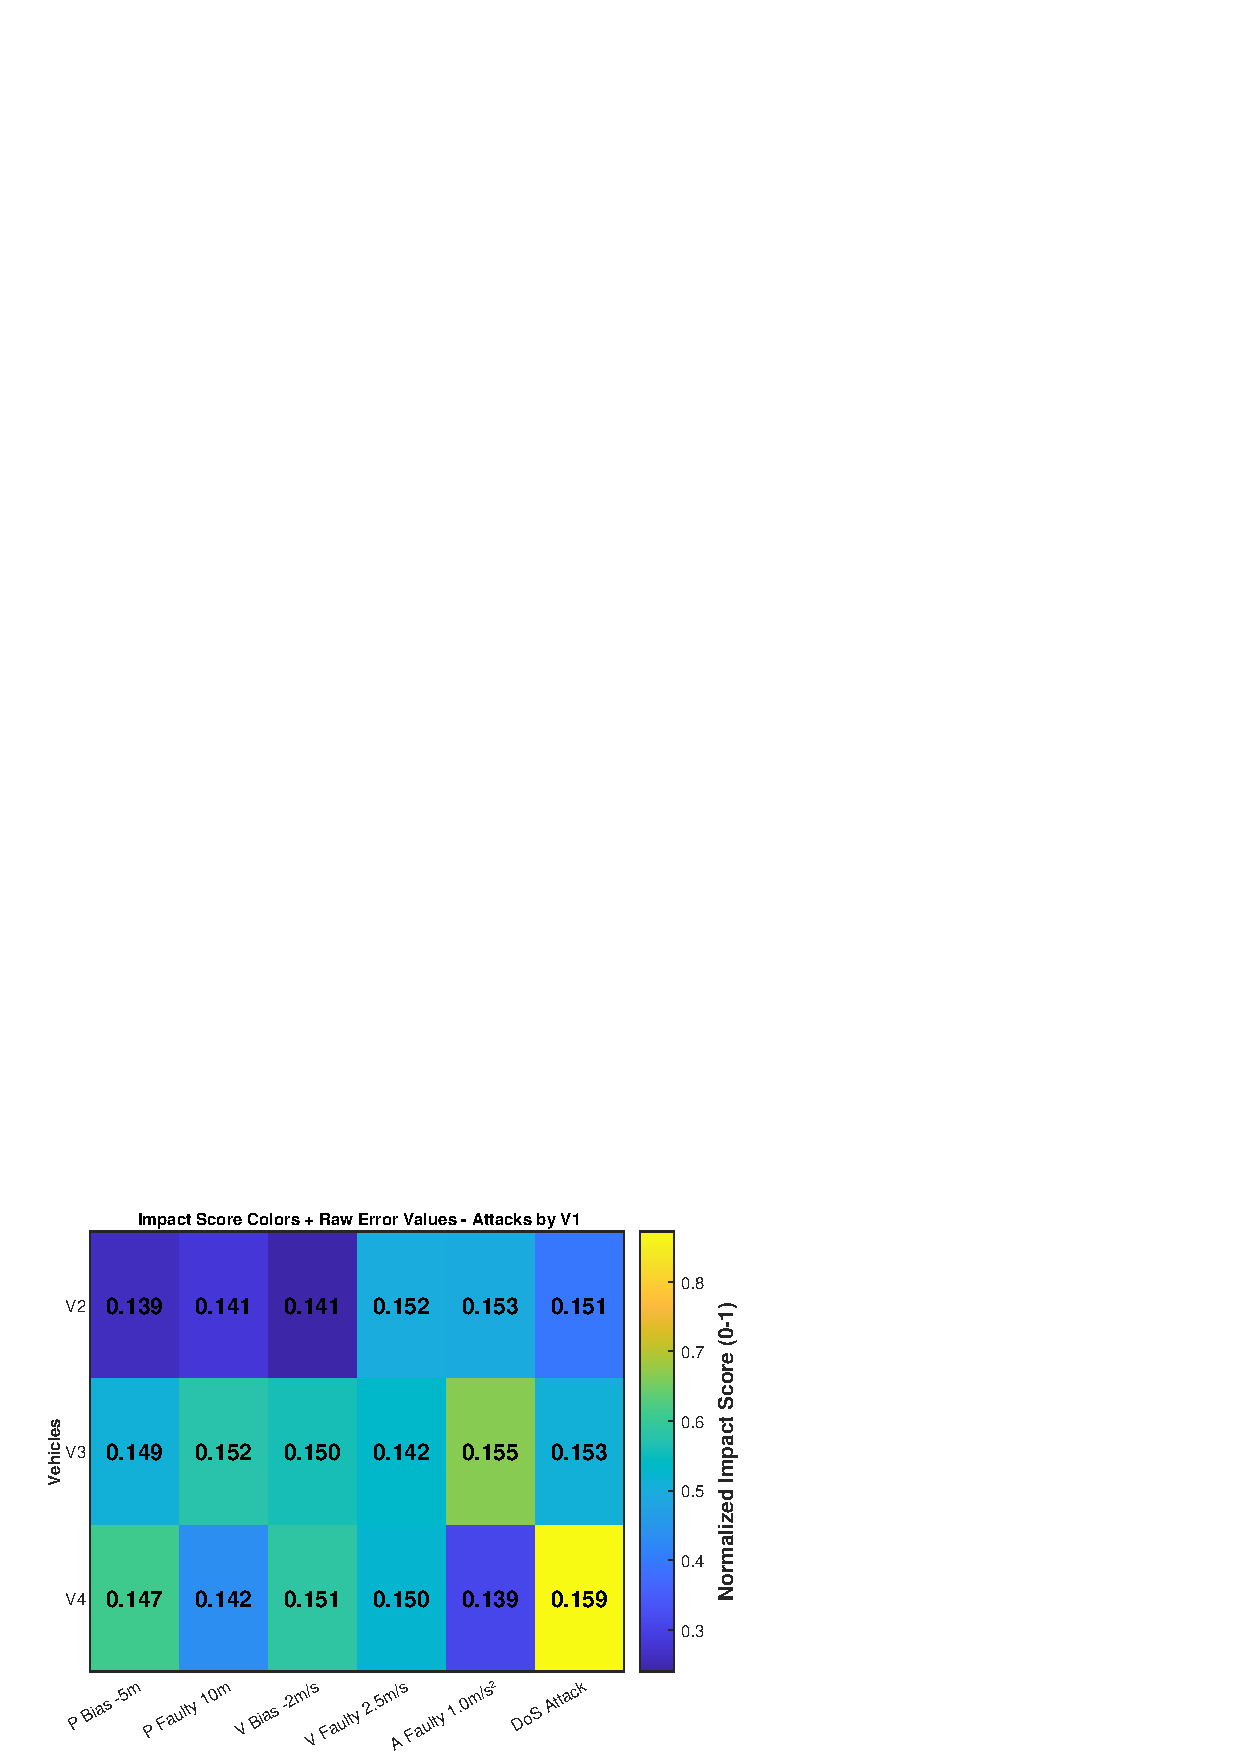
\includegraphics[width=\linewidth]{ch5/img/hybrid.jpg}
    \caption{Heatmap of normalized impact scores for all vehicles and attack cases.}
    \label{fig:hybird_heatmap}
\end{figure}


\begin{figure}[h!]
    \centering
    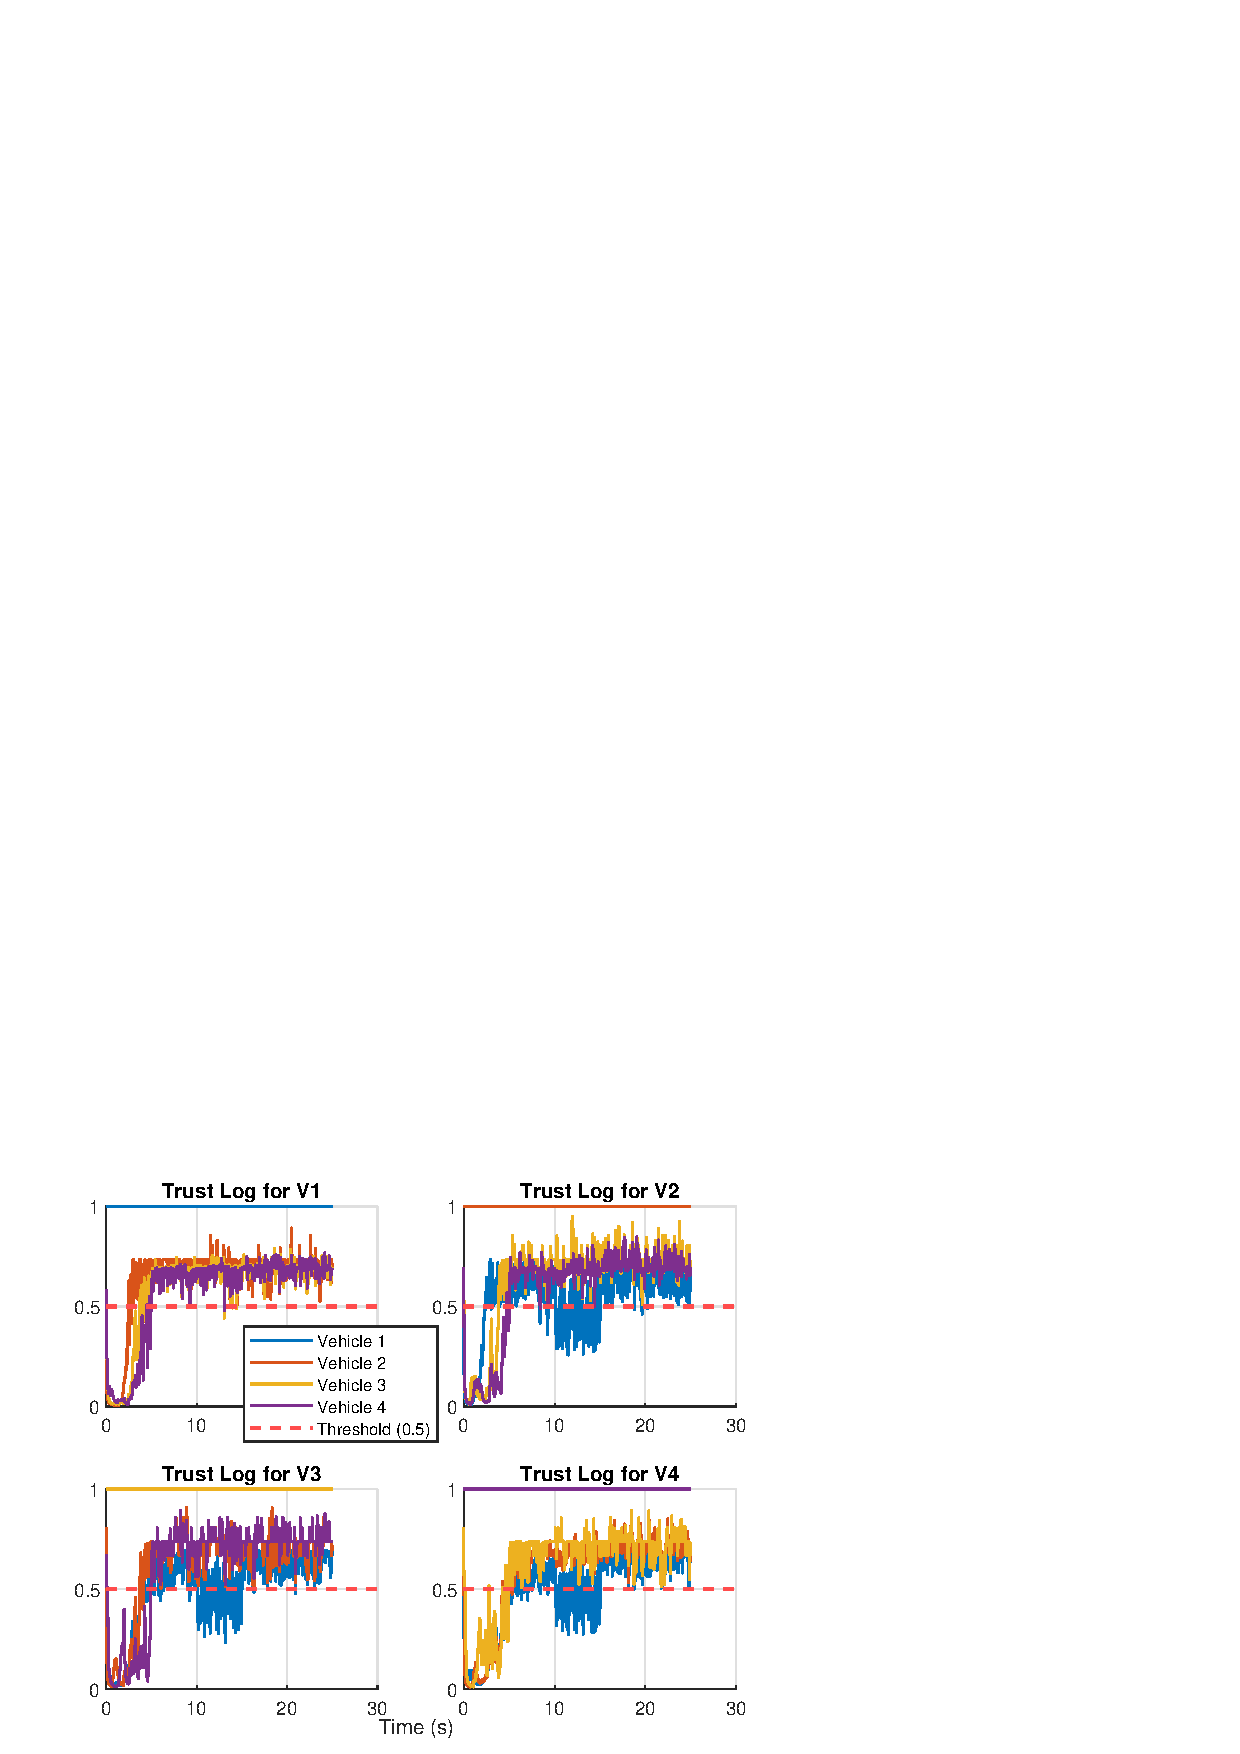
\includegraphics[width=\linewidth]{ch5/img/trust_all_new_huy.jpg}
    \caption{Trust score evolution during DoS attack ({\it\textbf{Case~6}}).}
    \label{fig:trust_Dos}
\end{figure}

In Figure~\ref{fig:trust_Dos}, the trust score evolution for the DoS attack (Case~6) is illustrated. During the attack period $[10, 15]$~s, these 3 vehicles (V2, V3, V4) exhibit a noticeable drop in trust values below the threshold of 0.5, indicating successful detection of the communication disruption. Once the attack ceases, the trust scores gradually recover, demonstrating the system ability to restore confidence and resume normal operation. This behavior confirms the effectiveness of the proposed trust mechanism in identifying and isolating malicious data in real time.






\subsection{Distributed State Estimation for Platoon Control}
% Introducing the platoon control framework using distributed state estimation
In this section, we present a platoon control framework that leverages distributed state estimation to enhance longitudinal control performance. The approach adopts a constant time headway spacing (CTHS) policy to maintain small inter-vehicle distances, improving traffic flow and safety. Two controllers are employed: an inner controller, based on the Intelligent Driver Model (IDM), for local longitudinal control using estimates from the local observer, and an outer controller, the Cooperative Adaptive Cruise Control (CACC), for distributed coordination using estimates from the distributed observer. These controllers are combined to form a robust final control strategy, balancing local responsiveness and platoon-wide consensus.

% Clarifying notation for state estimates
\subsubsection{Notation}

% For clarity, we define the notation for the estimated states used in the controllers:
% \begin{itemize}
%     \item \textbf{Local Observer ($\LO_i$)}: Each vehicle $i$ estimates its own state as $\hat{x}_0^{(i)} = [\hat{s}_0^{(i)}, \hat{v}_0^{(i)}, \hat{a}_0^{(i)}]^\top$, where $\hat{s}_0^{(i)}$, $\hat{v}_0^{(i)}$, and $\hat{a}_0^{(i)}$ are the estimated position, velocity, and acceleration of vehicle $i$, respectively.
%     \item \textbf{Distributed Observer ($\DO_i^{(j)}$)}: Each vehicle $i$ estimates the state of vehicle $j$ as $\hat{x}_i^{(j)} = [\hat{s}_i^{(j)}, \hat{v}_i^{(j)}, \hat{a}_i^{(j)}]^\top$, where $\hat{s}_i^{(j)}$, $\hat{v}_i^{(j)}$, and $\hat{a}_i^{(j)}$ are the estimated position, velocity, and acceleration of vehicle $j$ from the perspective of vehicle $i$.
% \end{itemize}

% Describing the inner controller: IDM
\subsubsection{Inner/Local Controller: Intelligent Driver Model (IDM)}
% Introducing the IDM and its purpose
The IDM is a car-following model that computes a vehicle's desired acceleration based on its own state and the relative state to its predecessor. Here, it serves as the inner controller for local longitudinal control, utilizing the local observer's estimate of the vehicle's own state, $\hat{x}_0^{(i)}$. The IDM acceleration for vehicle $i$ is given by:
\begin{equation}
    a_{\text{IDM},i} = \alpha \left[ 1 - \left( \frac{\hat{v}_0^{(i)}}{v_0} \right)^\delta - \left( \frac{s^*(\hat{v}_0^{(i)}, \Delta v_{i-1,i})}{s_{i-1,i}} \right)^2 \right],
\end{equation}
where:
\begin{itemize}
    \item $\hat{v}_0^{(i)}$ is the estimated velocity of vehicle $i$ from $\LO_i$.
    \item $s_{i-1,i} = s_{i-1} - s_i - L$ is the actual relative distance to the predecessor, with $L$ as the vehicle length (assuming direct sensor measurement for simplicity, as the query specifies IDM uses only local observer estimates, but relative distance typically requires predecessor data).
    \item $\Delta v_{i-1,i} = v_{i-1} - \hat{v}_0^{(i)}$ is the actual relative velocity, using the predecessor's true velocity $v_{i-1}$ from sensors.
    \item $s^*(\hat{v}_0^{(i)}, \Delta v_{i-1,i}) = s_0 + T \hat{v}_0^{(i)} + \frac{\hat{v}_0^{(i)} \Delta v_{i-1,i}}{2 \sqrt{\alpha \beta}}$ is the desired minimum gap.
    \item $\alpha$, $\beta$, $\delta$, $v_0$, $s_0$, and $T$ are model parameters: maximum acceleration, comfortable deceleration, free-flow exponent, desired velocity, minimum gap, and time headway, respectively.
\end{itemize}
% Noting the limitation and practical assumption
Since $\LO_i$ provides only $\hat{x}_0^{(i)}$ and not the predecessor's state, we assume vehicle $i$ uses sensor data (e.g., radar) for $s_{i-1,i}$ and $\Delta v_{i-1,i}$, consistent with standard IDM implementations, while adhering to the query's directive to use local observer estimates for the vehicle's own state.

% Describing the outer controller: CACC
\subsubsection{Cooperative Controller: Cooperative Adaptive Cruise Control (CACC)}
% Introducing the CACC and its cooperative purpose
The CACC enhances platoon coordination by leveraging information from multiple preceding vehicles via the distributed observer $\DO_{i}$. For vehicle $i$, the CACC control input is:
\begin{align}
    u_{\text{CACC},i}(k) = \sum_{j=1}^{i-1} [ \kappa_s \left( \hat{s}_i^{(j)}(k) - \hat{s}_0^{(i)}(k) - d_{i,j}(k) \right) \\ \notag +  \kappa_v \left( \hat{v}_i^{(j)}(k) -  \hat{v}_0^{(i)}(k) \right) + \kappa_a \left( \hat{a}_i^{(j)}(k) - \hat{a}_0^{(i)}(k) \right)]
\end{align}

where:
\begin{itemize}
    \item $\hat{s}_i^{(j)}(k)$, $\hat{v}_i^{(j)}(k)$, $\hat{a}_i^{(j)}(k)$ are the estimated position, velocity, and acceleration of vehicle $j$ from $\DO_i^{(j)}$.
    \item $\hat{s}_0^{(i)}(k)$, $\hat{v}_0^{(i)}(k)$, $\hat{a}_0^{(i)}(k)$ are the estimated position, velocity, and acceleration of vehicle $i$ from $\LO_i$ (included for consistency, though the query specifies distributed observer estimates for CACC).
    \item $d_{i,j}(k) = d + h \hat{v}_0^{(i)}(k)$ is the desired spacing between vehicles $i$ and $j$, with $d$ as a constant gap and $h$ as the time headway (for $j = i-1$, this aligns with the CTHS policy).
    \item $\kappa_s$, $\kappa_v$, $\kappa_a$ are control gains for position, velocity, and acceleration errors, respectively.
\end{itemize}
% Explaining the cooperative mechanism
This formulation ensures that vehicle $i$ adjusts its behavior based on the estimated states of all preceding vehicles, promoting consensus and stability across the platoon.

% Combining the controllers into a final strategy
\subsubsection{Final Controller}
% Defining the combined control input
The final control input integrates the IDM and CACC controllers to balance local and cooperative objectives. The target acceleration is:
\begin{equation}
    a_{\text{target},i} = (1 - \gamma(t)) a_{\text{IDM},i} + \gamma(t) u_{\text{CACC},i},
\end{equation}
where \(\gamma(t) \in [0,1]\) is a tuning parameter that is influenced by the opinion score mentioned in Section \ref{sec_trust_score}. For this context, we choose \(\gamma(t) = \min(\mathcal{O}_i)\).
% \begin{itemize}
%     \item $\gamma = 0$: Relies solely on IDM (local control).
%     \item $\gamma = 1$: Relies solely on CACC (cooperative control).
% \end{itemize}
% Applying a filter for smooth control
To prevent abrupt changes of the mixing 2 type controller, a first-order filter is applied:
\begin{equation}
    u_i(t) = u_i(t-1) + \tau_f (a_{\text{target},i} - u_i(t-1)),
\end{equation}
where $\tau_f$ is the filter time constant. 

% The vehicle's velocity is then updated as:
% \begin{equation}
%     v_i(t) = v_i(t-1) + u_i(t) \Delta t,
% \end{equation}
% with $\Delta t$ as the time step.

% Analyzing expected spacing for validation
\subsubsection{Expected Distance (Spacing)}
% Deriving steady-state spacing for evaluation
To validate the control strategy, we derive the expected steady-state spacing:
\begin{itemize}
    \item \textbf{IDM Steady-State Spacing}: When $a_{\text{IDM},i} = 0$ and $\Delta v_{i-1,i} = 0$:
    \[
    1 - \left( \frac{\hat{v}_0^{(i)}}{v_0} \right)^\delta = \left( \frac{s_0 + T \hat{v}_0^{(i)}}{s_{i-1,i}} \right)^2,
    \]
    yielding:
    \[
    s_{i-1,i} = \frac{s_0 + T \hat{v}_0^{(i)}}{\sqrt{1 - \left( \frac{\hat{v}_0^{(i)}}{v_0} \right)^\delta}}.
    \]
    \item \textbf{CACC Steady-State Spacing}: For the CTHS policy, when the platoon reaches consensus (all velocities equal), the spacing between vehicle $i$ and $i-1$ is:
    \[
    \boxed{s_i = d + \frac{h\,\hat{v}_0^{(i)}}{\,i-1}\,.}
    \]
\end{itemize}
% Explaining the validation process
These expressions allow comparison with simulation results, assessing the controllers' ability to maintain desired spacing under various conditions, including cyber-attacks.

\begin{figure}[h!]
    \centering
    \begin{subfigure}[t]{0.49\linewidth}
        \centering
        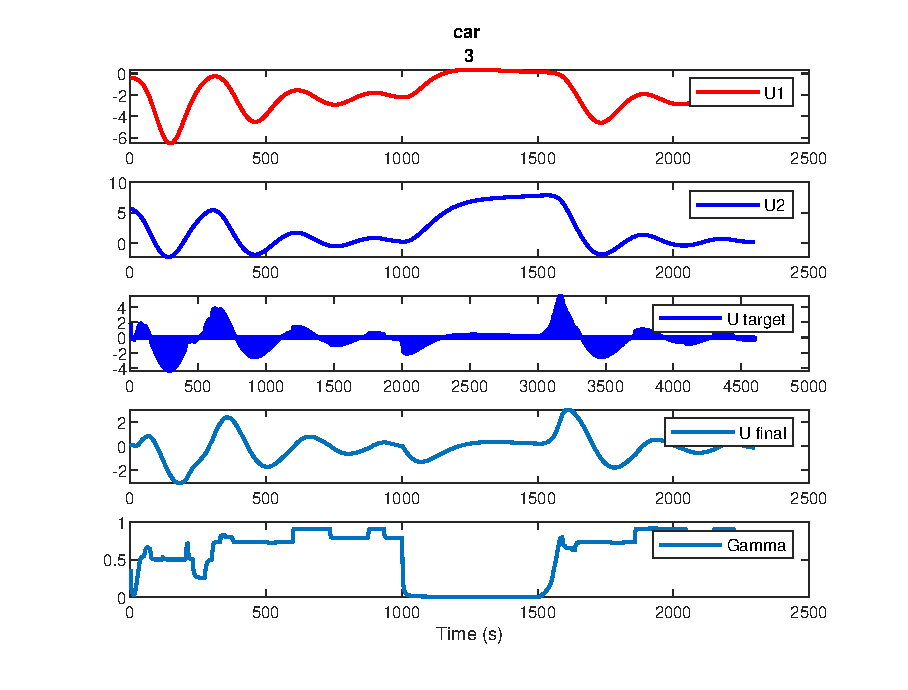
\includegraphics[width=1\linewidth]{ch5/img/controller_3.eps}
        % \caption{Compare with and without the local data exchange (Instance 1).}
        \label{fig:controller_3}
    \end{subfigure}
    \hfill
    \begin{subfigure}[t]{0.49\linewidth}
        \centering
        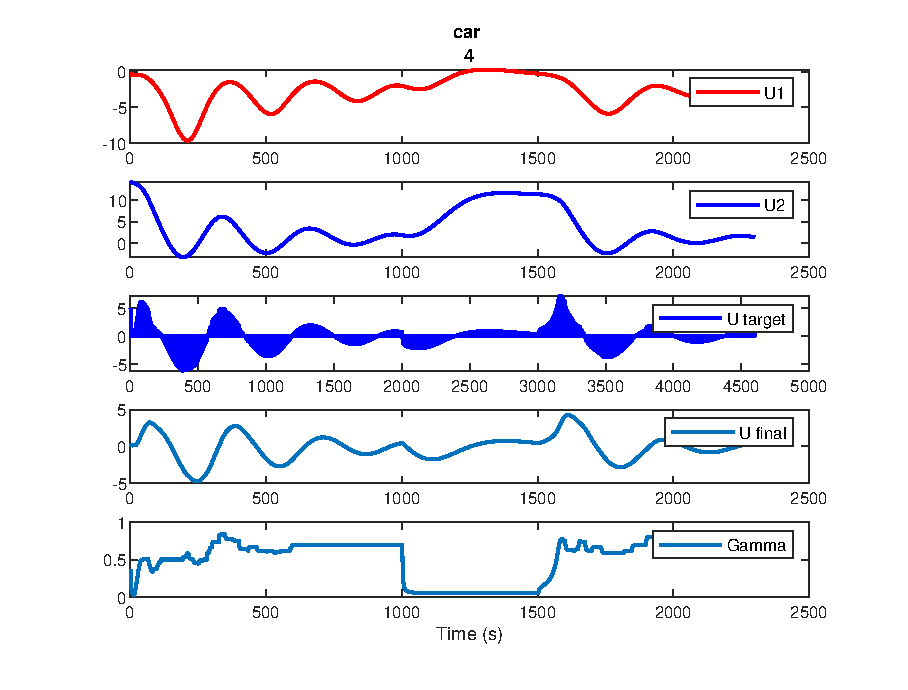
\includegraphics[width=1\linewidth]{ch5/img/controller_4.eps}
        % \caption{Compare with and without the local data exchange (Instance 2).}
        \label{fig:controller_4}
    \end{subfigure}
    
    \caption{Controller of vehicle 2 and 3.}
    \label{fig:controller_23}
\end{figure}


In figure \ref{fig:controller_23}, we can see the control input of vehicle 2 and 3, which is the acceleration of the vehicle. Smoothly switched between 2 controllers, and no abrupt change in the control input.
\begin{figure}
    \centering
    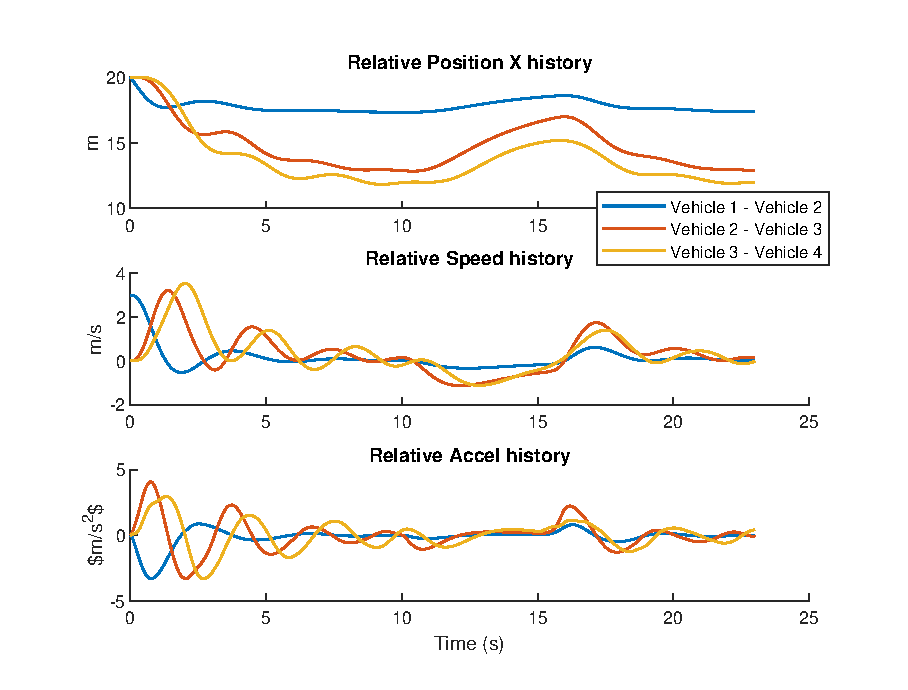
\includegraphics[width=0.8\linewidth]{ch5/img/relative_final_true.eps}
    \caption{Relative state of the vehicle in platoon}
    \label{fig:relative_final_true}
\end{figure}


In figure \ref{fig:relative_final_true}, we can see the relative state of the vehicle in platoon, which is the difference between the position of the vehicle and the position of its predecessor.
That prouve even in attack scenario, the vehicle can keep good distance No accident or crash happen in the platoon, which is a good sign of the robustness of the platoon control framework. 
Also that show the expected distance between the vehicle and its predecessor is maintained, which is the desired spacing in the platoon.


\section{Conclusion and Future Work}\label{sec_conclusion}
\vspace*{-0.2cm}
% Limitation – Estimating Malicious Vehicles
This paper presented a distributed observer-based platoon control framework capable of maintaining stability and safety under cyberattacks. The approach combines local and distributed observers with a trust evaluation mechanism to assess the reliability of inter-vehicle data, ensuring robust operation even with compromised nodes. 
%
%The proposed trust-based observer effectively protects the platoon by isolating malicious agents and preventing the propagation of corrupted data. However, it does not allow accurate estimation of the states of those malicious vehicles themselves. Once a vehicle's trust score falls below the threshold, its information is excluded from neighbor updates and is no longer corrected by trusted nodes. Consequently, its state estimate cannot converge to the true state. The framework thus prioritizes platoon safety and resilience over reconstructing the exact behavior of compromised vehicles a limitation shared by most existing distributed observer designs.
%

\subsection{Open Problems and Future Directions}
\vspace*{-0.2cm}
The analysis in this chapter focuses on stability and boundedness (ISS) under bounded disturbances and a trust-driven switching topology. Several open problems remain before such architectures can be made both sharper (less conservative) and more resilient in practice:
\begin{itemize}
    \item \textbf{Matrix-valued (channel-wise) trust weights.}
    In~\eqref{eq_observer}--\eqref{design_gain}, the coupling weights $w_{il}^{(j)}(t)$ are scalar and therefore apply the same attenuation to all state channels. A promising extension is to replace them with \emph{matrix} gains $W_{il}^{(j)}(t)\in\mathbb{R}^{n_x\times n_x}$ (e.g., diagonal or block-diagonal), allowing the trust mechanism to down-weight only the corrupted channels (e.g., acceleration) while preserving reliable channels (e.g., position). This leads to a matrix-weighted virtual Laplacian and stability conditions of the form
    $\|\mathcal{A}_{\mathrm{DO}}^{(j)}(t)\|_*\le \alpha<1$ for a suitably defined induced norm, or equivalently LMI-type contraction constraints on the lifted (block) error dynamics.

    \item \textbf{Trust/detection delay and rollback mechanisms.}
    In realistic networks, trust values are computed from time windows and may be delayed; consequently, false data can enter the distributed observer before a node is flagged, degrading the estimate. Moreover, abruptly cutting a node can temporarily reduce information flow and worsen estimation during the transition.
    A natural direction is to equip each host with a \emph{rollback buffer}: store a fixed window of past estimates and received packets. When the trust of a node drops below threshold, roll back to time $t-T_{\mathrm{w}}$ (window length) and re-propagate the observer using (i) only trusted neighbors and (ii) model-based prediction/local-observer anchoring to bridge the missing information. This resembles fixed-lag smoothing with trust-aware data rejection and could mitigate transient corruption while preserving stability, provided the reset/rollback map is bounded and updates satisfy a dwell-time or bounded-variation condition.

    \medskip
    \noindent\emph{Contamination rollback (compact recipe).}
    If a neighbor $l^{\star}$ is flagged at time $t$, undo the last $K$ steps by keeping a buffer of the \emph{innovation terms} appearing in~\eqref{eq_DO}. For each step $k$, store $\hat{x}_i^{(j)}(k)$ and
    \begin{align*}
    \eta_{il}^{(j)}(k) &\triangleq w_{il}^{(j)}(k)\big(\hat{x}_l^{(j)}(k)-\hat{x}_i^{(j)}(k)\big),\quad l\in\mathcal{N}_i,\\
    \eta_{i0}^{(j)}(k) &\triangleq w_{i0}^{(j)}(k)\big(\hat{x}_0^{(j)}(k)-\hat{x}_i^{(j)}(k)\big),
    \end{align*}
    as well as the input term $\hat{u}_j(k)$. When $l^{\star}$ is flagged, set $x\leftarrow\hat{x}_i^{(j)}(t-K)$ and replay for $k=t-K,\ldots,t-1$ using the same observer update but excluding $l^{\star}$ (or a malicious set $\mathcal{M}$):
    \begin{equation*}
    x \leftarrow A_{\text{b}}\Big(x + \sum_{l\in\mathcal{N}_i\setminus\mathcal{M}} \eta_{il}^{(j)}(k) + \eta_{i0}^{(j)}(k)\Big) + B_{\text{b}}\hat{u}_j(k),
    \end{equation*}
    and finally set $\hat{x}_i^{(j)}(t)\leftarrow x$.

    \item \textbf{Data-driven trust and learned uncertainty (with model-based safety layer).}
    Machine learning can be used to \emph{learn the mapping from signals to reliability}, while keeping the stability guarantee in the model-based layer by enforcing bounded weights. Concretely: (i) learn a calibrated trust score or anomaly probability from a feature vector built from innovation/residual signals (e.g., $\hat{x}_l^{(j)}-\hat{x}_i^{(j)}$, $\varepsilon_{i,l}^{(j)}$, packet age/loss, and consistency indicators), using change-point detection, self-supervised prediction, or lightweight sequence models; (ii) learn state-dependent covariance/uncertainty (heteroscedastic models) to adapt $\Sigma_{\text{local}}$ and thresholding; and (iii) implement the learned output only through a saturation/projection step that maps it to admissible weights satisfying Condition~(2) and preserving contraction in Condition~(3).
\end{itemize}

Future work will also focus on enhancing the trust mechanism by coupling it more closely with the controller, enabling trust evaluation for non-neighboring vehicles, and improving adaptability under dynamic communication topologies. 
We will also investigate machine-learning based trust estimation.
% \newpage
% \appendix